s\chapter{DNA and sequence alignment}
\label{chap1:DNA-align}
\section{Biological information is stored using DNA}
\label{sec:chap1:DNA}
\subsection{The molecule}
\label{sec:chap1:DNA-molecule}
The deoxyribonucleic acid (DNA) is the molecule that provides all
living organisms the ability to store, retrieve and pass from
generation to generation the genetic instructions required to make and
maintain a living organism. A molecule of DNA consists of two long
strands of complementary poly-nucleotide chains. The building blocks
which compose a chain of DNA are called nucleotides. The nucleoties are
molecules with simple structure composed of a five-carbon sugar, a
nitrogen-containing base and one or more phosphate groups (Figure
\ref{fig:chap1:nucleotide}a).

\begin{figure}[h]
	\begin{minipage}[b]{\linewidth}
	  \centering
	  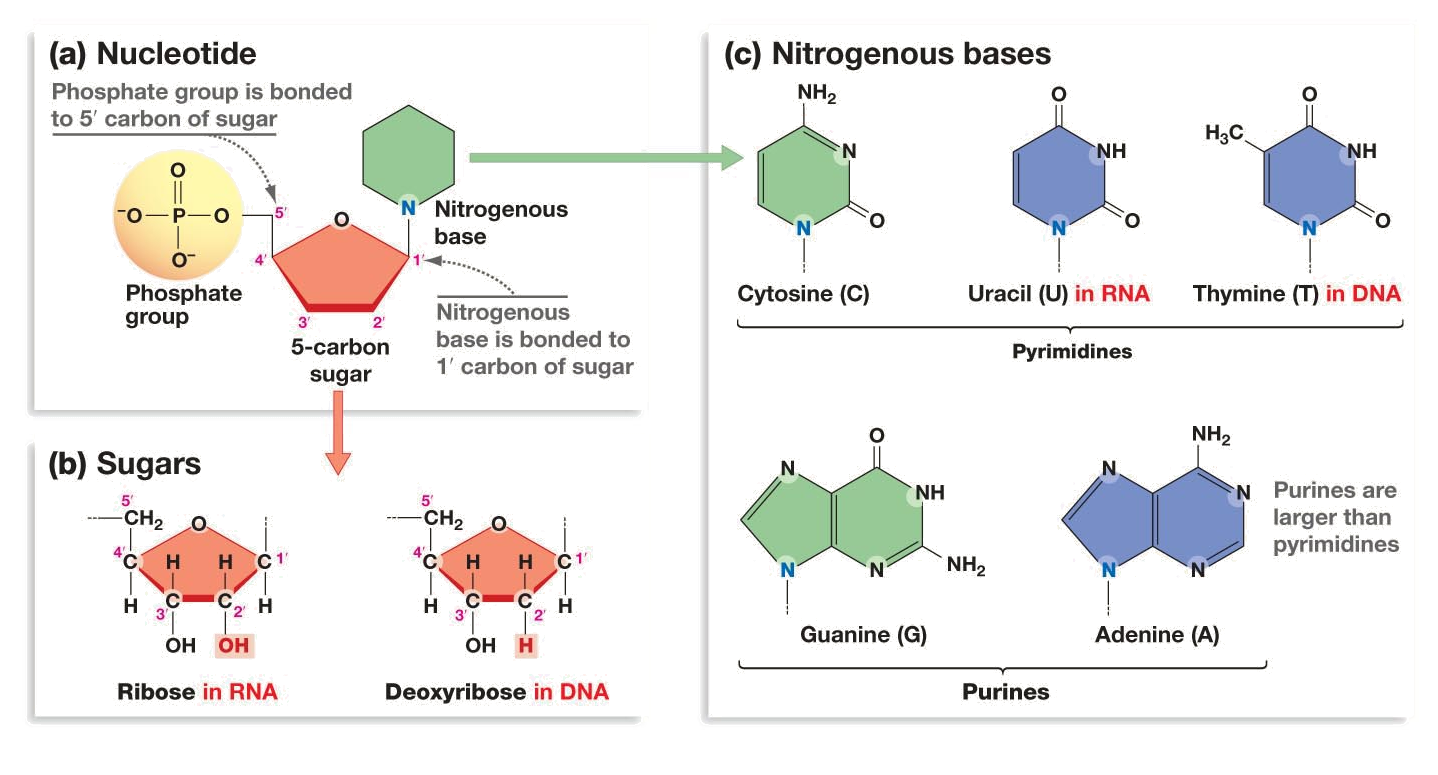
\includegraphics[width=\textwidth]{figures/chap1_nucleotide}
	  \caption{DNA molecule. a) DNA nucleotides are formed by a
       Phosphate group, a 5-carbon sugar and a nitrogenous base. b)
       Sugars from RNA/DNA differ by an OH/H group on the second
       carbon. c) The nitrogenous bases are Guanine, Adenine,
       Cytosine, Thymine (DNA only) and Uracil (RNA only).}
	  \label{fig:chap1:nucleotide}
   \end{minipage}
\end{figure}

The nucleotides are covalently linked together building a backbone
of sugar-phosphate bonds, in which the phosphate groups that are
attached to the 5th carbon of the sugars (5') form a covalent bond
with the 3rd carbon (3') of the next nucleotide in the strand (Figure
\ref{fig:chap1:dna_structure}). Following this fashion, DNA nucleotides can be enchained to form
an arbitrarily long DNA strands. Note that only one of the ends of a
DNA molecule will have a dangling phosphate group on its backbone (the 5' end),
giving an inherent polarity to the strand. The base group is the only
subunit that differs in each of the four types of nucleotides. There
are four different nitrogen-containing bases that give name to their
respecive nucleotide: Adenine (A), Thymine (T), Guanine (G) and
Cytosine (C) (Figure \ref{fig:chap1:nucleotide}c). The bases can hold together two strands of
DNA through hydrogen bonds. However, they do not pair at random: the
chemical structure of the bases only permits the efficient formation
of hydrogen bonds in the interior of the double helix between A and T
with 2 hydrogen bonds, and G and C with 3 hydrogen bonds. The latter 
pairing of bases is not a strict limitation. Nevertheless, in terms of
free energy, it's the best combination to bring the atoms close enough
to form hydrogen bonds without distorting the structure of the DNA
backbone. One last additional requirement to form the double helix
molecule is that the bases can only pair if the complementary strands
are antiparallel, i.e. the polarities of the strands (5' and 3') are
oriented in an opposed manner (see Figure
\ref{fig:chap1:dna_structure}).

\begin{figure}[h]
	\begin{minipage}[b]{\linewidth}
	  \centering
	  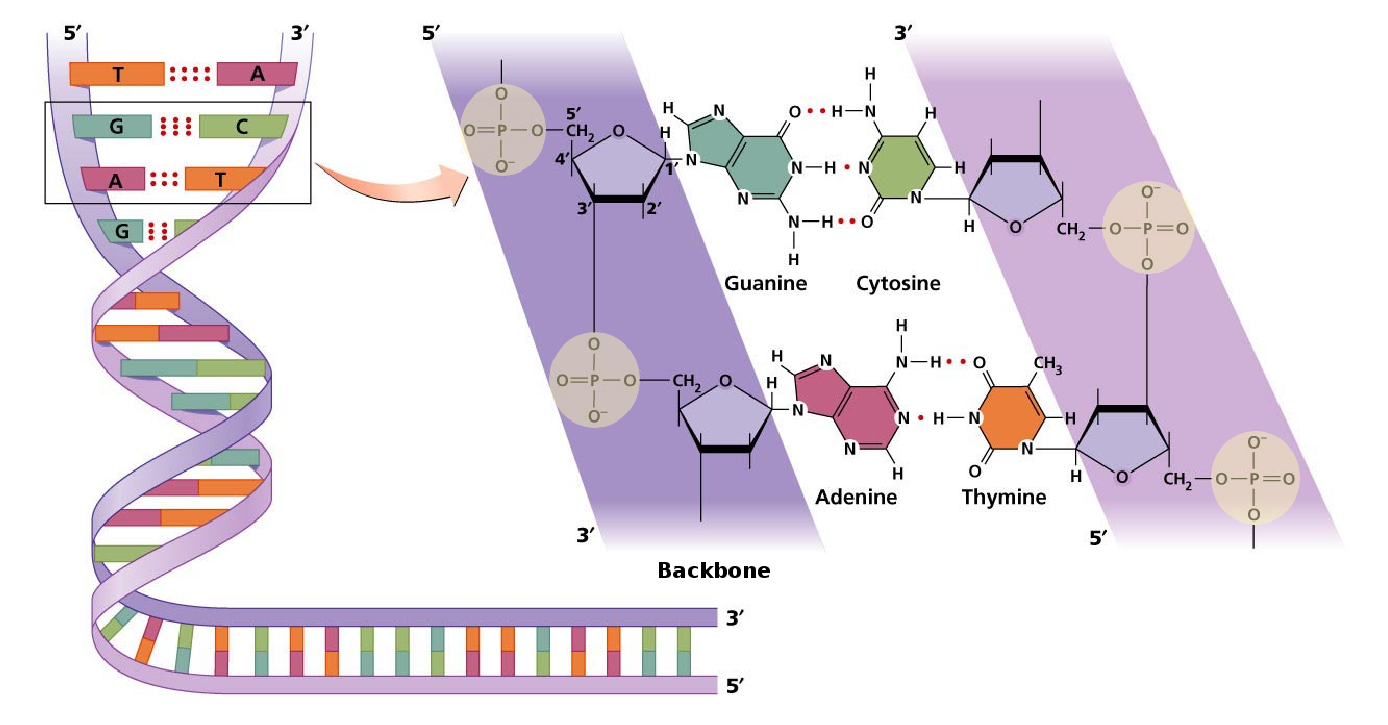
\includegraphics[width=\textwidth]{figures/chap1_dna_structure}
	  \caption{Structure of the DNA double helix. The nitrogenous bases
     hold together through hydrogen bonds: A and T with two bonds, C
     and G with three. The nucleotide pairs form stacks through
     sugar-phosphate bonds.}
	  \label{fig:chap1:dna_structure}
   \end{minipage}
\end{figure}


The discovery of the double helix structure of the DNA (Watson and
Crick ref) in 1953 was crucial to answer two important questions: (i)
how the information is stored in a chemical form and (ii) how this
information is passed from the mother cell to its daughters. The
answer to the first question is that the biological information in
living organisms is encoded in the sequence of nucleotides along DNA
strands. Therefore, the genetic information is analogous to a text
with a 4-letter alphabet: A, C, G and T. In consequence, different
organisms differ from each other because they have different
nucleotide sequences. The discovery of the DNA structure also shed
some light to the second question. The fact that the DNA molecule
contains two strands bearing identical information rapidly suggested
a mechanism of DNA replication: unwinding the two strands and filling
them separately with the complementary nucleotide sequence would give
rise to two new double stranded DNA molecules with the same information.

\subsection{Origins of DNA}
\label{sec:chap1:DNA-origins}
There are two main types of nucleic acids, which differ in the type of
sugar contained in their sugar-phosphate backbone (Figure \ref{fig:chap1:nucleotide}b). The acid based on
the sugar deoxyribose is known as deoxyribonucleic acid (DNA) and
contains the bases A, G, C and T
(Sec. \ref{sec:chap1:DNA-molecule}). On the other hand, the acid based
on sugar ribose, known as ribonucleic acid (RNA), contains the bases
A, C, G and Uracil (U), see
Figure. \ref{fig:chap1:nucleotide}c. Despite their structural
similarities, the RNA is commited to many more cellular tasks than its
sister nucleic acid. For instance, RNA is usually found in cells in the form of a
single-stranded molecule, whereas DNA is almost always in the form of
a double stranded polynucleotide chain. Being single stranded, the RNA
backbone is flexible, allowing the polymer chain to bend back on
itself and form weak bonds between different parts of the same
molecule. In fact, these types of internal associations form
specific shapes that are dictated by its sequence (Figure
\ref{fig:chap1:rna_enzyme}). The shape of the RNA molecule, in turn,
may recognize other molecules and bind to them selectively or act as a
catalyst in some chemical reactions. However, besides its enzymatic
roles, the RNA can also store and replicate genetic information in the same manner
as DNA. Most notably, RNA works in all living organisms as an
intermediate in the transfer of genetic information in the form of
messenger RNA (mRNA), bearing the information and guiding the
synthesis of proteins.

\begin{figure}[h]
	\begin{minipage}[b]{\linewidth}
	  \centering
	  \includegraphics*[width=0.6\textwidth]{figures/chap1_rna_enzyme_full}
	  \caption{Single-stranded RNA molecules can form secondary
       structures. a) Self-annealing of complementary nucleotides from
       the same RNA strand. b) Representation of the secondary
       structure. Source \cite{alberts}.}
	  \label{fig:chap1:rna_enzyme}
   \end{minipage}
\end{figure}

The triple role of RNA (enzymatic, protein synthesis and
information-bearing) strongly suggests that early stages of life
emerged from a combination of RNA and proteins. Such early RNA-protein
world would imply the existence of genetic code prior to DNA, which is
consistent with the ubiquitous use of messenger RNA (mRNA) and
transfer RNA (tRNA) as protein-building machinery. Given the success
of this early form of life, an immediate question arises: why would
the transition from RNA to DNA be so complete as to eradicate all
RNA-based genomes of living organisms? The straightforward answer is
that DNA genomes would have had substantial advantage with respect to
RNA genomes in terms of the
reliable production of progeny genotypes. In effect, the absence of
the $-OH$ group on desoxyribose renders DNA much more structurally
stable than RNA. In addition, the use of Thymine in place of Uracil
evades one of the most common sources of mutations in RNA: the accidental
production of Uracil via the deamination of Cytosine (see the
similarities in Figure \ref{fig:chap1:nucleotide}c). These advantages
for DNA-based organisms may have facilitated its survival in less permisive
environments where they could develop more complex biological functions.

\subsection{Genes and genomes}
\label{sec:chap1:DNA-genomes}

\begin{table}[h]
\centering
\caption{Genome size and protein-coding gene count of model organisms.}
\begin{tabular}{|l|c|c|}
	\hline
   {\bf Organism} & {\bf Genome size} [bp] & {\bf Coding genes} \\
   \hline
	{\em Escherichia coli} (Bacterium) & $4.6\cdot10^6$ & $\sim$4.400\\ \hline
	{\em Sacchromyces cerevisiae} (Yeast) & $12.5\cdot10^6$ &
   $\sim$6.000\\ \hline
	{\em Neurospora crassa} (Fungus) & $39.9\cdot10^6$ &
   $\sim$10.000\\ \hline
	{\em C. Elegans} (Nematode) & $100.2\cdot10^6$ &
   $\sim$20.000\\ \hline
	{\em Arabidopsis Thaliana} (Plant) & $135\cdot10^6$ & $\sim$27.000\\ \hline
	{\em Drosophila Melanogaster} (Fly) & $180\cdot10^6$ &
   $\sim$13.000\\ \hline
	{\em Danio Rerio} (Zebra Fish) & $1.7\cdot10^9$ & $\sim$26.000\\ \hline
	{\em Mus musculus} (Mouse) & $2.8\cdot10^9$ & $\sim$23.000\\ \hline
	{\em Homo Sapiens} (Human) & $3.3\cdot10^9$ & $\sim$20.000\\ \hline
\end{tabular}
\label{tab:chap1:genome-sizes}
\end{table}

In eukaryotic cells, the large amounts of DNA required to encode all
the information needed to sustain cellular life, are packaged into
{\bf chromosomes}. Chromosomes are very long double-stranded DNA
molecules found in the cell nucleous (Figure \ref{fig:chap1:chromosomes}). These DNA molecules fit
readily inside the nucleous and, after they are replicated, they can
be easily distributed between the two daughter cells. On the other
side, prokaryotic cells typically carry their genes on a single,
circular DNA molecule called {\em bacterial chromosome}, found in the cytoplasm.

\begin{figure}[h]
	\begin{minipage}[b]{\linewidth}
	  \centering
	  \includegraphics*[width=0.6\textwidth]{figures/chap1_chromosomes_full}
	  \caption{Human karyotype. Human cells have 23 pairs of
       chromosomes. Each cell contains two copies of chromosomes 1 to
       22 and two copies of chromosome X (female) or one copy of
       chromosome X and one copy of chromosome Y (male). Source \cite{alberts}.}
	  \label{fig:chap1:chromosomes}
   \end{minipage}
\end{figure}

The DNA in human species is packed into 24 different chromosomes, each
consisting of a fine thread of DNA and a set of proteins that fold and
pack it into a compact structure. Such complex of protein and DNA is
called {\bf chromatin}. The main function of the chromosomes is to carry
the genes (Figure \ref{fig:chap1:genes}). A gene is a segment of DNA that is transcribed, i.e. that
is converted to RNA either to be used as is (structural, catalytic,
regulatory RNA...) or to guide the synthesis of a protein. The 
total genetic information carried by all the chromosomes of an
organism constitutes its {\bf genome}. As it may be expected, there
exists a correlation between the genome size and the complexity of the
species, Table \ref{tab:chap1:genome-sizes} summarizes the genome sizes of the most widely used
model organisms.

\begin{figure}[h]
	\begin{minipage}[b]{\linewidth}
	  \centering
	  \includegraphics*[width=0.6\textwidth]{figures/chap1_genes_full}
	  \caption{Organization of genes in the human genome. a)
       Representation of chromosome 22. b) A ten-fold expansion of a
       fragment of chromosome 22 with about 40 genes indicated in
       red. c) An expanded portion of (b) showing four genes. d)
       Representation of one of the genes of chromosome 22 where the
       regulatory region and its 9 exons are indicated. Source
       \cite{alberts}.} 
	  \label{fig:chap1:genes}
   \end{minipage}
\end{figure}

\subsection{Evolution of genomes}
\label{sec:chap1:genome-evolution}

The evolution of the current living species from the ancestral forms
of life has been an impressive journey. The living organisms had been
continuosly adapting to get through the selective pressure of the
environment, a process that wouldn't have been possible without the
capacity of the genomes to change and {\em generate} new
genes. Remarkably, the genes that provide  an organism with selective
advantage do not arise as a whole; they are instead the product of
thousands or even millions of years of collection of non-deleterious
single nucleotide changes, combined with the {\em horizontal transfer} of
bigger sequence blocks. 

\begin{figure}[h]
	\begin{minipage}[b]{\linewidth}
	  \centering
	  \includegraphics*[width=0.6\textwidth]{figures/chap1_genome_content}
	  \caption{A representation of the nucleotide sequence content of
       the sequenced Human genome. Source \cite{alberts}.}
	  \label{fig:chap1:genome-content}
   \end{minipage}
\end{figure}

Single nucleotide changes or {\em mutations} may be produced by the
exposure to radiation, double-strand breaks on DNA, replication
errors, etc. However, the evolution of genomes due to single
mutations is an extremely slow process, considering that error rates
during DNA synthesis in humans are in the $10^{-6}$ to $10^{-8}$
range. Besides, only an insignificant part of such mutations will
remain, given that deleterious mutations are rapidly displaced by
selective pressure. On the other side, more sophisticated mechanisms,
which include: sequence duplication and recombination, virus
infections or plasmid transformation, among others, allow the transfer
of bigger blocks of DNA, a process called horizontal gene
transfer (HGT). As a result of HGT, the genomes of the more complex
species are full of duplicated sequences that may belong, for instane,
to a functional substructure present in many genes, a massive
infection from ancestral virus or an accidental duplication. Such
repeated sequences are so significant that fill up to 50\% of the
Human genome, whereas the protein coding sequences only represent the
2\% (Figure \ref{fig:chap1:genome-content}). We will see in the
following chapters that such repetitive structure of the genomes
is the major source of difficulties in the field of sequence mapping.

\subsection{DNA sequencing technologies}
\label{sec:chap1:DNA-sequencing}
DNA sequencing is a method or technology that is used to measure the
precise order of the four bases (A,C,G,T) in a strand of DNA. The
first sequencings methods: {\em Chemical} and {\em Sanger} sequencing
were invented in 1977. These methods were very slow and expensive,
requiring enormous human power, but were able to generate reads of
several hundreds of nucleotides (Sanger). Later in the early 2000's,
{\em Next Generation sequencing technologies} were developed,
currently yielding bilions of reads in less than 24 hours. A summary
of the current sequencing technologies along with their properties is
presented in Table \ref{tab:chap1:sequencing}.

\begin{table}[h]
\centering
\caption{DNA sequencing technologies in current use.}
\begin{tabular}{|l|c|c|c|c|c|}
	\hline
   {\bf Name} & {\bf Read length} [bp] & {\bf Reads} & {\bf
     Time} & {\bf Error rate} & {\bf Cost/Mb} \\
   \hline
   {\em Illumina} & 150+150bp & $>$100M & 24hrs & $\sim$1\% & 0.1\$ \\ \hline
   {\em PacBIO} & up to 30kbp & $\sim$100K & 1-4hrs & $\sim$15\% &
   0.5\$ \\ \hline
   {\em Pyrosequencing} & 700bp & 1M & 24hrs & $<$1\% & 10\$ \\ \hline
   {\em SOLiD} & 50+50bp & 1G & 1 week & $<$0.5\% & 0.1\$ \\ \hline
   {\em Sanger} & 900bp & $<$100 & hours & $<$0.1\% & 2000\$ \\ \hline
\end{tabular}
\label{tab:chap1:sequencing}
\end{table}


\section{Sequence alignment and mapping}
\label{sec:chap1:mapping}
In this section we will define two important concepts for this work:
sequence alignment and sequence mapping. {\em Sequence alignment} is a
process in which sequences of DNA, RNA or protein are arranged to
identify the regions of highest similarity based on a score model. In
other words, alignments are measurements of similarities between
sequences. Alignments can be {\em local} or {\em global}, depending on
whether subsequences of the query sequence are expected to be found
split in distinct regions along the reference (local alignment) or the query sequence is
expected to be found as a whole (global alignment). An example of a {\em
  local} alignment would be to align the mRNA sequence of a gene that
contains introns against its reference genome, whereas {\em global}
alignments would be used to align sequences of DNA that have been
extracted from the genome itself. On the other side, {\em sequence
  mapping} is the process of finding the most probable original locus
of a short sequence in a much larger reference, e.g. its reference
genome. In the following sections we describe and discuss the
complexity and purpose of some basic algorithms used for sequence
alignment and mapping.  

\subsection{Alignment algorithms}
\label{sec:chap1:align}
Despite there is a myriad of sequence alignment algorithms in the
literature, the vast majority are based on the same approach: {\em
  dynamic programming} methods. The alignment between two sequences is
computed by applying a recurrence 
relation throughout a matrix of $mn$ terms, called {\em edit matrix}
or {\em alignment matrix},
where $m$ and $n$ are the respective sequence lengths. Such relation
is based on a substitution matrix, the {\em score matrix}, that
establishes a relationship between the possible sequence modifications
and their respective penalties. The technique of dynamic programming
can be applied to produce {\em global alignments} via the {\em
Needleman-Wunsch} algorithm, and {\em local alignments} via the
{\em Smith-Waterman} algorithm, described below.
\subsubsection{Needleman-Wunsch algorithm}
\label{sec:chap1:align-nw}
The Needleman-Wunsch algorithm is used to compute the {\em global distance}
between two sequences. Let $q$ be a query sequence and
$t$ be the reference sequence, with lengths $m$ and $n$,
respectively. Hence, the alignment matrix
$S$ is an integer matrix with dimensions $m \times n$, i.e. $S \in
\mathbb{Z}^{m \times n}$. We will refer to the $i$-th character of
either sequence with a subindex, i.e. as $t_i$ and $q_i$. Let us also
introduce a simple score matrix, which defines the update values for
character match, mismatch, gap open and gap extend (Table
\ref{tab:chap1:align-score}).

\begin{table}[h]
\centering
\caption{Examples of alignment scores.}
\begin{tabular}{|l|c|c|}
   \hline
    & {\bf Levenshtein} & {\bf bwa-mem}\\
   \hline
	$P_m$ (match) & $0$ & $-1$\\ \hline
	$P_s$ (mismatch) & $1$ & $4$\\ \hline
	$P_o$ (gap open) & $1$ & $6$\\ \hline
	$P_e$ (gap extend) & $1$ & $1$\\ \hline
\end{tabular}
\label{tab:chap1:align-score}
\end{table}

Other, more sophisticated matrices, take into account the probability
of nucleotide transition (or aminoacid, in case of protein) drawn
from empirical models of sequence evolution (Figure
\ref{fig:chap1:blosum-matrix}).

\begin{figure}[h]
	\begin{minipage}[b]{\linewidth}
	  \centering
	  \includegraphics*[width=0.6\textwidth]{figures/chap1_blosum_matrix}
	  \caption{BLOSUM62 matrix, used to score alignments between
       evolutionarily divergent protein sequences.}
	  \label{fig:chap1:blosum-matrix}
   \end{minipage}
\end{figure}

Once the score matrix is defined, the Needleman-Wunsch algorithm
is initialized as follows: each character of the query sequence $q_i$ is
associated with the $i+1$-th row, similarly the reference characters
$t_i$ are placed one per column, following the same trend. The first row
and column are not associated to any character because they represent
the first run of gaps. Hence, the first row and column are
initialized by recursively applying a gap extension penalty $P_e$, as
shown in Figure \ref{fig:chap1:nw-init}.

\begin{figure}[h]
	\begin{minipage}[b]{\linewidth}
	  \centering
	  \includegraphics*[width=0.35\textwidth]{figures/chap1_nw_init}
	  \caption{Initialization of a Needleman-Wunsch alignment between
       \texttt{ATGCAA} and \texttt{ACGCTTTAA}.}
	  \label{fig:chap1:nw-init}
   \end{minipage}
\end{figure}


Then, the matrix cells are computed row-wise or column-wise starting
from the top left corner with the following update rules:

\begin{equation}
  \label{eq:chap1:nw-update}
  S[i,j] = \begin{cases}
    S[i-1,j-1] + P_m, & \text{if $q_i = t_j$}.\\
    \mbox{min}(S[i-1,j-1] + P_m,S[i-1,j] + P_e,S[i,j-1]+P_e), & \text{if
    $q_i \neq t_j$ and gap is open}. \\
    \mbox{min}(S[i-1,j-1] + P_m,S[i-1,j] + P_o,S[i,j-1]+P_o),
    & \text{otherwise}. \\
 \end{cases}
\end{equation}

\begin{figure}[!h]
	\begin{minipage}[b]{\linewidth}
	  \centering
	  \includegraphics*[width=0.8\textwidth]{figures/chap1_nw_alignments}
	  \caption{Needleman-Wunsch matrix for $q=$\texttt{ATGCAA} and
       $t=$\texttt{ACGCTTTAA} (top row) and alignment path based on
       backtracking through valid cell transitions (bottom
       row). Green: match/mismatch. Red: Gap open/extend. \textbf{a)}
       Score matrix for Levenshtein distance 
       ($P_m=0$, $P_s=1$, $P_o=1$, $P_e=1$). \textbf{b)} Score matrix
       for $P_m=-1$, $P_s=4$, $P_o=6$, $P_e=1$. }
	  \label{fig:chap1:nw-alignments}
   \end{minipage}
\end{figure}

Applying \eqref{eq:chap1:nw-update} for $q=$\texttt{ATGCAAA} and
$t=$\texttt{ACGCTTTAAA}, one obtains the matrix shown in Figure
\ref{fig:chap1:nw-alignments}. The final score of the alignment corresponds
to the value of the bottom-right cell (highlighted in red). The small
lines connecting adjacent cells represent the transitions that satisfy
the update rules.

The final alignment is computed following the transition trace from the
last cell back to the upper-left corner. Any path that connects these
two cells through valid transitions represents a valid best alignment
(Figure \ref{fig:chap1:nw-alignments}, second row). Note that
different score  models may produce different alignments. For
instance, the alignment of \texttt{AAATCA} against \texttt{AAAGAATTCA}
generates the best alignments represented in Table
\ref{tab:chap1:alignment-gaps}. In this example, the {\em bwa-mem}
score would be preferred because it produces only one alignment in
which all the gaps appear in succession.

\begin{table}[h]
\centering
\caption{Alignments generated with different score
  models for $q=$ \texttt{AAATCA} and $t=$ \texttt{AAAGAATTCA}.}
\begin{tabular}{|c|c|}
   \hline
   {\bf Levenshtein score} & {\bf bwa-mem score}\\
   \hline
   \texttt{AAAGAATTCA} & \texttt{AAAGAATTCA}\\
   \hline
	\texttt{--A-AA-TCA} & \texttt{AAA----TCA}\\
	\texttt{-A--AA-TCA} & \\
	\texttt{A---AA-TCA} & \\
	\texttt{AA--A--TCA} & \\
	\texttt{AA--A-T-CA} & \\
	\texttt{AAA---T-CA} & \\
	... & \\
   \hline
\end{tabular}
\label{tab:chap1:alignment-gaps}
\end{table}

\subsubsection{Smith-Waterman}
\label{sec:chap1:align-sw}
The Smith-Waterman algorithm is a simple variant of the
Needleman-Wunsch to compute local alignments. Local alignment is
preferred when the query sequence is much smaller, partially present
or split in the reference. For instance, the alignment of a mRNA
sequence against its full gene sequence. The exons will be aligned
{\em   locally}, each producing an independent score that will not be
affected by the low score of the intronic region gaps. On the other
side, a global alignment will report a low score given the huge amount
of gaps that would need to be introduced to fill the introns.

\begin{figure}[h]
	\begin{minipage}[b]{\linewidth}
	  \centering
	  \includegraphics*[width=0.65\textwidth]{figures/chap1_sw_init}
	  \caption{Smith-Waterman matrix initialization for $q=$\texttt{ATGCAA} and
       $t=$\texttt{TGTGCATGGAAAGCAGCT}.}
	  \label{fig:chap1:sw-init}
   \end{minipage}
\end{figure}


Smith-Waterman and Needleman-Wunsch are very similar methods, both use
the same matrix and the same update rules, however there are two
differences between them. First, the initial gap runs are initialized
with all 0 (Figure \ref{fig:chap1:sw-init}). Second, since this method
computes local alignments, the final score for a given
alignment may not coincide with the lower-right corner. Hence, one
should define a criterion to select good alignments. Usually, the
criterion is to select scores greater than some threshold with a
minimum alignment path length, e.g. match score greater than 30
(matrix score -30 with {\em bwa-mem} score model) and alignments
of, at least, 30 nucleotides. An example of a local alignment using
Smith-Waterman along with the best 3 local alignments is shown in
Figure \ref{fig:chap1:sw-alignments}. 

\begin{figure}[h]
	\begin{minipage}[b]{\linewidth}
	  \centering
	  \includegraphics*[width=0.65\textwidth]{figures/chap1_sw_alignments}
	  \caption{Smith-Waterman alignment for $q=$\texttt{ATGCAA} and
       $t=$\texttt{TGTGCATGGAAAGCAGCT} using {\em bwa-mem} score model.}
	  \label{fig:chap1:sw-alignments}
   \end{minipage}
\end{figure}


\chapter{Finding needles in a haystack}
\label{chap2:mapping}
\section{Sequence mapping}
\label{sec:chap1:seed}
\subsubsection{Mapping: formal definition}
Let $t$ and $q$ be sequences of DNA (e.g. a genome and a sequencing
read) of lengths $m$ and $n$, respectively. The alphabet of $t$ and
$q$ will be denoted as $\Sigma$ and contains the four DNA nucleotides
plus the unknown base \texttt{N}, $\Sigma = \{\texttt{A,C,G,T,N}\}$. Let $a_i$ denote
the 1-based $i$-th nucleotide of an arbitrary sequence $a$, and
$a_{i,j}$ its substring of $j-i$ nucleotides starting at position $i$,
e.g. if $a=$~\texttt{ACGGCAGTAT}, $a_2=$~\texttt{C} and
$a_{5,9}=$~\texttt{CAGT}. We then define the mapping process as:

\begin{equation}
  \label{eq:chap2:mapping-function}
  l = \min\limits_{j}(S_{qt}[n,j])
\end{equation}

where $S_{qt}$ is the Smith-Waterman alignment matrix of the
query sequence $q$ against the reference $t$. In other words, mapping
is the process of finding the position(s) $l$ on the reference for which
the local alignment between $q$ and $t_{l-n,l}$ yields the best
score.

\subsubsection{Aligning the fast way}
In Chapter \ref{chap1:DNA-align} we reviewed the basic alignment
algorithms. These algorithms solve elegantly the alignment problem and
allow us to find similarities between sequences, like conserved
regions of a protein in diverging species. In this section, however,
we will present methods with the aim of finding {\em where} a short
sequence aligns well in a much larger reference text
(eq. \eqref{eq:chap2:mapping-function}). Speaking in numbers, the
typical length of a high-throughput seqeuencing read is on the order of
hundreds of nucleotides (Table \ref{tab:chap1:sequencing}), whereas
the size of the reference (human genome) is over $10^9$ nucleotides
long (Table \ref{tab:chap1:genome-sizes}). In such a context, one could
use the Smith-Waterman algorithm to find the matrix positions $l$ that
satisfy the equation \eqref{eq:chap2:mapping-function} with complexity
$O(nm)$. Running this process in a modern computer takes around ten
seconds. This is a  reasonable performance if one needs to map several
reads, but recall that an Illumina MiSeq run yields more than 200 milion
reads in less than 24 hours (Table \ref{tab:chap1:sequencing}). Hence,
aligning a full lane with this method would take longer than 60 years.

To deal with this bottleneck, it is possible to query the genome at a
much faster rate using {\em indexes}. An index is a data structure
generated from the reference sequence that allows very fast sequence
lookup operations, e.g. the faster indexes require only $O(1)$ or
$O(n)$  (the length of the query) operations per lookup. This means
that, spending only a few number of operations, one may obtain the
complete list of positions in the reference where the query sequence is
present. However, an index only allows lookups of exact
sequences. Recall from Table \ref{tab:chap1:sequencing} that
high-throughput sequencing technologies have error rates ranging between
1\% and 15\%. Therefore it seems unlikely to find high-throughput
sequencing reads of hundreds of nucleotides without any
mismatch. Concretely, for a read of 100~nt and an error rate of 1\%,
and considering a binomial distribution of the errors, the probability
of finding a perfect read is:
\begin{equation}
  \label{eq:chap2:perfect_prob}
  P_{perfect}(n=100\mbox{ nt}, P_e=0.01) = (1-P_e)^n = 0.37
\end{equation}

In effect, looking for exact matches of 100~nt would work only in 37\%
of the reads. Instead of querying the index with the aim of finding
long exact matches, we use a method called {\em seeding}. This method
consists in looking up short subsequences of the query sequence $q$ to
maximize the probability of finding a perfect match, because short
sequences are less likely to contain mutations. However, one has to be
conservative and avoid extremely short sequences because these will
appear frequently in the reference and yield too many candidate
loci. In general, assuming a random genome of length $m$, the lookup
of a sequence of length $l$ yields $m/4^l$ matching loci. As the
lookup length increases, the number of reported loci reduces
exponentially. Seeding methods allow us to quickly find tentative
positions in the reference where the query sequence may align well. The
seeding step is then followed by local alignments of the whole query
sequence at all the candidate loci. Since the seed length is adjusted
to yield only a few matches in the genome, the positions of the best
alignments are found much faster than in a global Smith-Waterman
alignment.

\begin{figure}[h]
	\begin{minipage}[b]{\linewidth}
	  \centering
	  \includegraphics*[width=0.8\textwidth]{figures/chap2_stick_breaking}
	  \caption{Representation of error free subsequences modeled as a
       stick breaking problem. The mismatched nucleotides and the
       longest error-free stretch are highlighted in red.}
	  \label{fig:chap2:stick_breaking}
   \end{minipage}
\end{figure}

Although it is fast, the seeding method is an heuristic. This means
that there is a certain probability of missing the best aligning
position $l$. For instance, imagine that we split the sequence in
Figure \ref{fig:chap2:stick_breaking} in two halves (seeds) of 30
nucleotides. Since the sequence contains two mutations (highlighted in
red), each in one seed, neither seed will be found exactly in the
reference. Or even worse, the mutated seed sequence may casually exist
in the reference and report a locus different than the real position
where the query sequence was taken from.

We can model the probability of successful seeding, which is the
probability of selecting a subsequence of $q$ without any
mutation. The probability depends on the global error
rate\footnote{This accounts for the technology error rate, the 
  divergence between the sequenced organism and the reference genome
  and the rate of single nucleotide polymorphisms (SNP).},
the length of the query sequence and the error distribution, that will
be assumed binomial. Consider that the sequencing read $q$ was extracted
from $t$ and modified with respect to the original reference at $k$
positions. Inserting the $k$ differences in the read at random would
produce $k+1$ subsequences without errors. This process is analogous
to inserting $k$ breaks at random in a stick of length $n$. Figure
\ref{fig:chap2:stick_breaking} illustrates the concept for a read of
length $n=60$ and $k=2$, the longest error-free stretch is highlighted
in red. For a fixed binomial distribution of errors with $q=1-p$, the
cummulative distribution of the longest error-free stretch $X_m$ from
a read of length $m$ is: 

\begin{equation}
\label{eq:chap2:longest-run}
  P(X_m \leq x) = \sum_{k=0}^{m}
  \left( \begin{array}{c}
    m \\ k
  \end{array}
  \right)
  q^k p^{m-k} P \left(
  Z_k \leq \frac{x}{m-k}
  \right)
\end{equation}

where

\begin{equation}
  P (Z_k \leq x) = \sum_{j=0}^{k+1}
  \left( \begin{array}{c}
    k+1 \\ j
  \end{array} \right)
  (-1)^j(1-jx)^k_+
\end{equation}

is the cummulative distribution of the longest fragment when inserting
$k$ breaks ($a_+ = a$ if $a>0$ and $0$ otherwise). The cummulative
distribution of the seeding probability \eqref{eq:chap2:longest-run}
is represented in Figure \ref{fig:chap2:seedprob} for $q=0.02$ and
several read lengths.

\begin{figure}[h]
	\begin{minipage}[b]{\linewidth}
	  \centering
	  \includegraphics*[width=0.8\textwidth]{figures/chap2_seedprob}
	  \caption{Seeding probability for error rate $q=0.02$ and read
       lenghts $m=25,50,75,100,125,150$~nt.}
	  \label{fig:chap2:seedprob}
   \end{minipage}
\end{figure}

A good tradeoff for the seed length on Illumina reads from Homo
Sapiens is between 17 and 20 nucleotides. With these seed lengths, the
expected number of perfect matches in the reference is
$3\cdot10^9/4^{17} < 1$, with a seeding probability over 95\%
(Figure \ref{fig:chap2:seedprob}) even with reads as short as 50 nucleotides.

\section{Efficient string search structures}
\label{sec:chap2:index}
In the following subsections we will review the most common data
structures (indices) used to efficiently search on long reference
texts. The goal of an index structure is to provide very fast lookup
operations over a reference text with complexities of $O(1)$ or $O(n)$
and memory footprint $O(m)$ (comparable to the raw genome size).

\subsection{Hash tables}
\label{sec:chap2:index-hash}
The first and simplest indexing technique is based in hash tables. The
idea is simple, build a hash table with all the substrings in $t$ of
fixed length $l$:
\begin{equation}
  H\{t_{i,i+l}\} = [H\{t_{i,i+l}\}, i] \qquad \mbox{for } x=1\ldots m-l
\end{equation}
where $H\{\cdot\}$ is the hash table and $\cdot$ is the table key. Note
that the seed length is fixed in this index and this restricts the
search to sequences of length $l$. Therefore, each hash table is built
for a concrete error rate and sequence length. Note also that the
arbitrary substring $t_{i,i+l}$ may be repeated in different positions
of the reference, therefore we use the array append operation $a = [a,
  \cdot]$ to keep a complete list of the positions matching $t_{i,i+l}$.
Storing all the $l$-mers in a hash table achieves the fastest lookup
time $O(1)$, with a good memory footprint of $O(m)$. However, the
fact that $l$ is determined at the building time and cannot be
modified is a major drawback, especially when the error rate is
variable or unknown. Nonetheless, querying seeds of length $l'<l$ is
possible by appending all the combinations of sequence termination,
yielding a lookup cost of $O(4^{l-l'})$.

\subsection{Trees}
Another possible index structure is the tree of suffixes. A tree
is nothing but the tree-structure arrangement of all the suffixes of
the reference text. If $t$ is our reference text of length $m$, then
the $i$-th suffix is the end of $t$ starting from position $i$,
i.e. $t_{i,m+1}$, and will be denoted as $t_{i,}$.

A tree structure is built using nodes that contain links to other
nodes, called {\em branches}. Each node has as many branches as the
cardinality of the alphabet $\|\Sigma\|$. The suffixes are added to
the tree starting always from the same node, the {\em root}. The
different {\em leaves} of the tree represent all the suffixes of
the text. The tree is built following the procedure illustrated in
figure \ref{fig:chap2:tree}. To insert the suffix $t_{i,}$, the root node is
selected, if the branch $t_i$ does not exist, a new node is added to
this branch. Then, the same process is recursively applied starting at
the new node and following $t_{i+1}$. The starting position of the
suffix $i$ is stored at the last node of the branch, i.e. the {\em leaf}.

\begin{figure}[h]
	\begin{minipage}[b]{\linewidth}
	  \centering
	  \includegraphics*[width=0.8\textwidth]{figures/chap2_suffix_tree}
	  \caption{Process of construction of a tree structure containing
       all the suffixes of the text \texttt{ATGAC}. The starting
       position of the suffixes are stored in the leaf nodes.}
	  \label{fig:chap2:tree}
   \end{minipage}
\end{figure}

To lookup all the occurrences of a seed in the index, the branches
corresponding to the nucleotides of the seed are followed. If, during
this process, a branch is not found, the sequence is not present in
the reference. Otherwise, the seed search will probably terminate in
an intermediate node, then all the branches downstream must be
followed to retreive the starting positions of the seed in the
text. If the suffixes are stored at full, this last process will
become very demanding and the tree will have a footprint of
$O(m^2)$. Therefore, the suffixes are usually pruned at a predefined
length $l$. 

The tree structure has a worse overall performance and size compared to
the hash table. Assuming that the tree is pruned at length $l$, each
query has a cost $O(l)$ and the memory footprint is asymptotically
$O(lm)$. However, when querying subseeds of length $l'<l$, the cost is
$O(4^{l-l'})$ only in the worst case, because only the existing seed
terminations (branches) will be followed. Another implementations of
the tree structure called {\em suffix tree} (cite SuffixTree) stores
more than one letter per branch and reuses repeated parts of the text
to compact the structure, achieving $O(m)$ space and $O(m)$ access
time.

\subsection{Suffix arrays}
\label{sec:chap2:seed-sa}
The suffix array (cite Myers) is a powerful data structure used to
index and compress big texts. It is an array containing the start
positions of all the text suffixes sorted in lexicographical order. In
other words, the suffix array of a text $t$ of length $m$ is:
\begin{equation} 
\label{eq:chap2:suffix-array}
\mbox{SA}_t = [i_1, i_2, \ldots, i_m] \qquad \mbox{where} \qquad t_{i_j,} < t_{i_k,}
\mbox{ iif } j<k. 
\end{equation}
in equation \eqref{eq:chap2:suffix-array}, the symbol $<$ denotes the
lexicographical order comparison between two suffixes. Before
computing the suffix array, the lexicographically smallest symbol
(usually \$) must be appended at the end of the text. Therefore, $t_m
= \$$.

An example of the suffix array of \texttt{GATGCGAGAGATG} is shown
in Figure \ref{fig:chap2:suffix_array}. Note that
$t=$\texttt{GATGCGAGAGATG\$} and $m=14$. The list of numbers at the
top of Figure \ref{fig:chap2:suffix_array} is the suffix array and the
corresponding suffixes for each position are shown below.

\begin{figure}[h]
	\begin{minipage}[b]{\linewidth}
	  \centering
	  \includegraphics*[width=0.6\textwidth]{figures/chap2_suffix_array}
	  \caption{.}
	  \label{fig:chap2:suffix_array}
   \end{minipage}
\end{figure}

Noteworthy, the suffix array can be computed by traversing the {\em
  suffix tree} from left (branch \texttt{AAAA...A}) to right (branch \texttt{TTTT...T}). The positions stored at each leaf
coincide with the indices stored at the suffix array.

We can use the suffix array to query exact sequences to the
text. Since the suffixes are sorted, one possible method is to use the
bisection algorithm on the suffix array, which takes $O(\log_2 m)$ for
a query $q$ of {\bf any} length. The memory footprint is compact, taking
only $O(m)$ space.

\subsection{BW Transform and FM index}
\label{sec:chap2:seed-bwt}
\subsubsection{Burrows-Wheeler Transform}

The Burrows-Wheeler Transform (BWT) is a lossless text transform based
on text permutation (cite BW-transform). The transform of a text $t$ of
length $m$ will be denoted as $\mbox{BW}_t=\mbox{BWT}(t)$. The BWT is performed in
two steps: (i) Compute the suffix array of $t$,
i.e. $\mbox{SA}_t$. (ii) The BWT of $t$ is the preceding character of
each suffix array position. Formally, 
\begin{equation}
  \mbox{BW}_t[i] = t[\mbox{SA}_t[i]-1]
\end{equation}
for $\mbox{SA}_t[i] > 1$ and $\mbox{BW}_t[i] = t[m]$ if
$\mbox{SA}_t[i] = 1$.

Following the previous example of Figure \ref{fig:chap2:suffix_array},
we construct the Burrows-Wheeler transform by taking the preceding
character of each suffix (Figure \ref{fig:chap2:bwt_sa}). A
fundamental property of the Burrows-Wheeler transform is the fact that
the set of the same characters in the BWT appear in the same relative
order as in the Suffix Array. That means that the first \texttt{A} in
the BWT will be also the first \texttt{A} appearing in the SA,
i.e. they both refer to the same position in the original text.

\begin{figure}[h]
	\begin{minipage}[b]{\linewidth}
	  \centering
	  \includegraphics*[width=0.6\textwidth]{figures/chap2_bwt_sa}
	  \caption{.}
	  \label{fig:chap2:bwt_sa}
   \end{minipage}
\end{figure}

To prove this property, consider the first character of the BWT shown
in Figure \ref{fig:chap2:bwt_sa}, $\mbox{BW}_t[1] =$ \texttt{G}. Note
that the full suffix starting at this position is the text
concatenation of $\mbox{BW}_t[1]$ and the suffix
$t_{\mbox{SA}_t[1],}$. Since $t_{\mbox{SA}_t[i],} >
t_{\mbox{SA}_t[j],}$ for any $j>i$, $\mbox{BW}_t[1] =$ \texttt{G} will
be also the first \texttt{G} to appear in the suffix array. The
property is illustrated in Figure \ref{fig:chap2:bwt_order}.

\begin{figure}[h]
	\begin{minipage}[b]{\linewidth}
	  \centering
	  \includegraphics*[width=0.6\textwidth]{figures/chap2_bwt_order}
	  \caption{.}
	  \label{fig:chap2:bwt_order}
   \end{minipage}
\end{figure}

The Burrows Wheeler transform has other interesting properties, like
the rearrangement of the text into runs of similar characters. This
allows for effective text compression using simple algorithms like
run-length encoding.

\subsubsection{The Ferrangina-Manzini Index and Backward Search}

The Burrows-Wheeler transform is an interesting structure but it
cannot be used as is for the purpose of sequence mapping. The
Ferrangina-Manzini (FM) index (cite FM-index) is a combination of the
BWT with other structures that allows to query any sequence $q$ of
length $n$ in $O(n)$ time, regardless of the text size. 

Let us illustrate how the Burrows-Wheeler transformed text can be used
to look for an arbitrary sequence $q$ in the text, for instance, $q =$
\texttt{GAGA} (Figure \ref{fig:chap2:backward_search}). All the
occurrences of \texttt{GAGA} in the text end with \texttt{A}. Each
\texttt{A} is also the first letter of some suffix of the
text. Because such suffixes all start with \texttt{A}, they are stored
next to each other in the suffix array, namely between positions 2 and
5 (Figure \ref{fig:chap2:backward_search}). However, only those
suffixes preceded by a \texttt{G} can potentially contain the
query. This is exactly the information encoded in the Burrows-Wheeler
transformed text $\mbox{BW}_t$. In this concrete example, all the
\texttt{A}s are preceded by a \texttt{G}, so the text contains 4
suffixes that start with \texttt{GA}.

\begin{figure}[h]
	\begin{minipage}[b]{\linewidth}
	  \centering
	  \includegraphics*[width=0.6\textwidth]{figures/chap2_backward_search}
	  \caption{.}
	  \label{fig:chap2:backward_search}
   \end{minipage}
\end{figure}

So far we know there are 4 suffixes in the text that start with
\texttt{GA}, but how do we continue extending the query? Now we need
to search for all the \texttt{A}s preceding the suffix
\texttt{GA}. Indeed, we just learned that the \texttt{G}s from the
suffix \texttt{GA} are the 2nd, the 3rd, the 4th and 5th on the
BWT. Therefore, they also will be the 2nd, 3rd, 4th and 5th \texttt{G}
in the Suffix Array. So now we can continue from the range in the SA
covering from the 2nd until the 5th \texttt{G}, and check for the
preceding \texttt{A}s in the BWT. Now we find two \texttt{A}s that
correspond to the 1st and 2nd \texttt{A} in the Suffix array. We would
continue in the same fashion until the completion of the query
$q$. This process is called {\em\bf backward search} because the query
starts with the last nucleotide and iteratively queries the preceding
nucleotides.

The BWT is necessary but not sufficient to perform the backward search
on an index. We need additional information to: (i) get the ranges of
each nucleotide in the suffix array and (ii) counting the order of
occurrence of each nucleotide in the BWT.

Since the Suffix Array is a representation of the sorted suffixes, all
the occurrences of the same letter will appear together, i.e. first
all the \texttt{A}, then all the \texttt{C}, and so on (Figure
\ref{fig:chap2:suffix_array}). Therefore, it will be enough to store
the position of the first appearance of each letter in an array
$C$. It is straightforward to retrieve the full range of any
nucleotide from $C$, for instance the range of \texttt{A} is
$C[\texttt{A}]$ to $C[\texttt{C}]-1$. In general, the full range of
the $i$-th letter of the alphabet $\Sigma$ is $[C[\Sigma[i],
    C[\Sigma[i+1]-1]]$.  

To store the order of occurrence of the nucleotides in the BWT we will
use a structure called $Occ$. This structure, shown in Figure
\ref{fig:chap2:bs_occ_c}, is the individual cummulative count of each
nucleotide in the BWT. Using the cummulative count, we can now the 
current order of a nucleotide in any position of the BWT or the order
of the nucleotides appearing in a range of the BWT.

\begin{figure}[h]
	\begin{minipage}[b]{\linewidth}
	  \centering
	  \includegraphics*[width=0.6\textwidth]{figures/chap2_bs_occ_c}
	  \caption{.}
	  \label{fig:chap2:bs_occ_c}
   \end{minipage}
\end{figure}


Figure \ref{fig:chap2:bs_occ_c} illustrates the query of $q =$
\texttt{GAGA} in $t$, now using the complete index with $C$ and
$Occ$. First we start looking for the full range of \texttt{A}, this
is from $C[\texttt{A}]$ until $C[\texttt{C}]-1$. Then we check the
occurrences of \texttt{G} within this range: right before the range
there is only one \texttt{G},
i.e. $Occ(\texttt{G},C[\texttt{A}]-1)=1$, and at the end of the range
we have $Occ(\texttt{G},C[\texttt{C}]-1)=5$, therefore the range
contains 4 \texttt{G}, from the 2nd until the 5th. Then we would like
to obtain the range covering these \texttt{G}s. Since $C[\texttt{G}]$
points to the 1st \texttt{G}, our target range is $C[\texttt{G}] + 1$
until $C[\texttt{G}] + 4$. Then we can start again the process looking
for the {\em Occ}urrences of the next nucleotide in the query.

In general, we define the range update process for an arbitrary query
$q$ of length $n$ as
\begin{equation}
  \label{eq:chap2:bs_update}
  \begin{array}{c}
  sp[i+1] = C[q[n-i]] + Occ(q[n-i],sp[i] - 1) \\
  ep[i+1] = C[q[n-i]] + Occ(q[n-i],ep[i]) - 1
  \end{array}
\end{equation}
for $i = 1 \ldots n-1$ and $sp[0] = C[q[n]]$, $ep[0] =
C[q[n]+1]-1$. In this update model, the range at the $i$-th step of
the query is $[sp[i], ep[i]]$, therefore $sp$ and $ep$ denote the
start and end points of the BWT ranges, respectively. Once the update
process finishes, we obtain a range $[sp[n],ep[n]]$. The number of
occurrences of the query $q$ in the text will be equal to
$ep[n]-sp[n]+1$ and their positions will be the values of the Suffix
Array from $sp[n]$ to $ep[n]$. Note that the update algorithm
described in \eqref{eq:chap2:bs_update} takes exactly $n$ update steps
and that we only need the Suffix Array, the $Occ$ table and the $C$
array. Hence, we conclude that the backward search algorithm has a
complexity of $O(n)$. The memory footprints for the different
structures are: $O(m)$ for the Suffix Array, $O(\|\Sigma\|)$ for the
$C$ array and $O(\|\Sigma\|m)$ for the $Occ$ table, resulting in an
overall memory footprint $O(\|\Sigma\|m)$. However, for DNA texts and
using simple compressing techniques, the final size of the index may
be reduced to less than $m$ bytes.

\subsubsection{Bi-directional FM index}
There exists a variant of the FM-index that supports both {\em
 backward} and {\em forward} search, as well as switching from
backward search to forward search, or vice versa. This index is 
called {\bf bi-directional FM index}. This index is just an extension
of the {\em FM index} described above, in which the reverse complement
of the text is appended to the original text. That is, if $t$ is the
original text to be indexed and $({\cdot})^R$ denotes the reverse
complement operation, then the input to the FM index is
``$tt^R\$$''. The main advantages of having the reverse complement
of the text stored in the index are:
\begin{itemize}
\item the possibility of searching
in both DNA strands with just one query.
\item performing a {\em backward search} operation on the reverse
  strand is equivalent to a {\em forward search} on the forward
  strand, and vice versa.
\end{itemize}
For that, we need to know the position of the start and end pointers
for both strands for a given query, e.g. if we perform a backward
search of \texttt{ACTGCA} and compute its {\em sp} and {\em ep}
pointers in a given index using \eqref{eq:chap2:bs_update}, the
pointers of the reverse complement of the query (reverse strand)
$sp_{q^R}$ and $rp_{q^R}$ are necessary to perform bi-directional search.

To keep track of the positions of the pointers in the forward query
and its reverse complement, we define the following property: 
\begin{property}
  \label{property:chap2:interval_size}
  For any given sequence $q$, the number of occurrences of $q$ and
  $q^R$ on a bi-directional FM index structure is the same.
\end{property}

As an example, we will search the query \texttt{ACTGCA} starting
from the middle, i.e first do backward search on \texttt{ACT} and then
extend the query forward querying \texttt{GCA}. We start the
backward search with the nucleotide \texttt{T}. We need to store the
pointers both for the forward and reverse complement of the query. For
the first nucleotide this process is straightforward; we find the {\em
  sp} and {\em ep} pointers as: $sp_{\texttt{T}} = C[$\texttt{T}$]$,
$ep_{\texttt{T}} = C[$\texttt{T}$+1]-1$. And the same for the reverse
complement: $sp_{\texttt{T}^R}=C[$\texttt{T}$^R]=C[$\texttt{A}$]$ and
$ep_{\texttt{T}^R}=C[$\texttt{A}$+1]-1$. Since we know from the
Property \ref{property:chap2:interval_size} that
$ep_q-sp_q=ep_{q^R}-sp_{q^R}$, we do not need to store the four
pointers. 

A search state in the bi-directional search index is completely
defined by a triplet: the forward pointer $fp_q = sp_q$, the reverse
pointer $rp_q=sp_{q^R}$ and the interval size $sz_q =
ep_q-sp_q+1$. Using this notation, we derive a second property:

\begin{property}
  \label{property:chap2:interval_complement}
  For any given sequence $q$, $fp_q = rp_{q^R}$ on a bi-directional FM
  index structure.
\end{property}

Once the triplet $fp_{\texttt{T}}, rp_{\texttt{T}}, sz_{\texttt{T}}$
has been computed, one can extend the search either forward or
backward. To continue with our example, we extend the forward strand
of the query backwards, adding a \texttt{C}. We do so with the
backward search update step described in
\eqref{eq:chap2:bs_update}. This will yield the updated values
$fp_{\texttt{CT}}$ and $sz_{\texttt{CT}}$, but we still need to keep
simultaneous track of the pointer in the reverse complement strand:
$rp_{\texttt{CT}}$. Note that a backward extension on the
forward strand is equivalent to a forward extension on the reverse
strand (the equivalent search of \texttt{CT} in the reverse strand is
\texttt{AG}). Thus, to know $rp_{\texttt{CT}}$ we need to perform
a forward search of the nucleotide \texttt{G} on the reverse strand of
the query. The process to update $rp_{\texttt{T}}$ to
$rp_{\texttt{CT}}$ relies on very basic properties of the
bi-directional FM index and the suffix array. Our current interval
$I_{\texttt{T}^R}=[rp_{\texttt{T}}, rp_{\texttt{T}}+sz_{\texttt{T}}-1]$ are all the
positions of the suffix array with suffixes starting with
$\texttt{T}^R=\texttt{A}$ (Figure \ref{fig:chap2:bs_occ_c}). Since the
forward-extended suffix \texttt{AG} also contains the suffix
\texttt{A}, the new pointer $rp_{\texttt{CT}}$ must lie in the current
interval $I_{\texttt{T}^R}$, i.e. $I_{\texttt{CT}^R} =
[rp_{\texttt{CT}}, rp_{\texttt{CT}}+sz_{\texttt{CT}}-1]$ is a
subinterval of $I_{\texttt{T}^R}$. More generally, we can divide any
interval $I_q$ in 5 subintervals, one for each possible forward
extension: $I_{q\texttt{A}}$, $I_{q\texttt{C}}$, $I_{q\texttt{G}}$,
$I_{q\texttt{T}}$ and $I_{q\texttt{N}}$, as shown in Figure
\ref{fig:chap2:forward_search}.  
\begin{figure}[h]
	\begin{minipage}[b]{\linewidth}
	  \centering
	  \includegraphics*[width=0.3\textwidth]{figures/chap2_forward_search}
	  \caption{.}
	  \label{fig:chap2:forward_search}
   \end{minipage}
\end{figure}
In such context, the following identities verify:
\begin{equation} 
  \begin{array}{c}
  I_q = I_{q\texttt{A}} \cup I_{q\texttt{C}} \cup I_{q\texttt{G}} \cup
  I_{q\texttt{T}} \cup I_{q\texttt{N}} \\
  |I_{q}| = |I_{q\texttt{A}}|+|I_{q\texttt{C}}|+|I_{q\texttt{G}}|+|I_{q\texttt{T}}|+|I_{q\texttt{N}}|
  \end{array}
\end{equation}
where $|I_q| = sz_{q}$. Provided that $sz_{\texttt{CT}} =
sz_{\texttt{AG}}$ from Property \ref{property:chap2:interval_size}, we
can obtain the interval sizes for the forward extension as
$|I_{q\texttt{X}}| = sz_{q\texttt{X}} = sz_{(q\texttt{X})^R} =
sz_{\texttt{X}^Rq^R}$, therefore the sizes obtained with the backward
search can be reutilized to compute the subinterval sizes
\begin{equation}
  \label{eq:chap2:interval_size}
  |I_{q\texttt{X}}| = sz_{\texttt{X}^Rq^R}
\end{equation}
where $\texttt{N}^R = \texttt{N}$. Once the subinterval sizes are
known, we use Property \ref{property:chap2:interval_complement} to
derive the update rules for $rp_{q}$: 
\begin{equation}
  \label{eq:chap2:forward_update}
  \begin{array}{c}
    rp_{\texttt{T}q} = rp_{q} \\
    rp_{\texttt{G}q} = rp_{q} + sz_{\texttt{T}q} \\
    rp_{\texttt{C}q} = rp_{q} + sz_{\texttt{T}q} + sz_{\texttt{G}q}\\
    rp_{\texttt{A}q} = rp_{q} + sz_{\texttt{T}q} + sz_{\texttt{G}q} +
    sz_{\texttt{C}q} \\
    rp_{\texttt{N}q} = rp_{q} + sz_{\texttt{T}q} + sz_{\texttt{G}q} +
    sz_{\texttt{C}q} + sz_{\texttt{A}q} \\
  \end{array}
\end{equation}

Back to our example, we already computed $fp_{\texttt{CT}}$ and
$sz_{\texttt{CT}}$ with the backward search update rules, we can now
follow Equation \ref{eq:chap2:forward_update} and obtain the reverse
strand query pointer as $rp_{\texttt{CT}} = rp_{\texttt{T}} +
sz_{\texttt{T}q} + sz_{\texttt{G}q}$.

To perform a forward search, one only needs to apply the same
procedure to the reverse strand. In effect, assume that we already
computed the triplet $fp_{\texttt{ACT}}$, $rp_{\texttt{ACT}}$,
$sz_{\texttt{ACT}}$ for the first half of the query. Now we would like
to continue extending the query (\texttt{ACTGCA}) forward, so we
perform a forward extension of \texttt{G} in the forward
strand. Again, performing a forward extension on the forward strand is
equivalent to a backward extension to the reverse strand, so we only
need to apply the same process but swapping the strands. We update the
reverse pointer $rp_{\texttt{ACTG}} = fp_{\texttt{CAGT}}$ with a backward search on
$\texttt{G}^R = \texttt{C}$ and compute the forward pointer as
$fp_{\texttt{ACTG}}=fp_{\texttt{ACT}}+sz_{\texttt{ACTA}}+sz_{\texttt{ACTC}}$.


\section{The sequence neighborhood}
\label{sec:neighborhood}
In this section we will introduce the concepts of sequence
neighborhood and neighbor sequences. The neighbor annotation of a text
$t$ will be very useful to determine sequence similarities and will
be exploited in some steps of the mapping algorithm to speed-up the
process and improve the quality of the classification.

Let us first define the {\bf sequence neighborhood}. A $k$-neighborhood is
the complete set of sequences that are $k$ nucleotides long, i.e. the
permutation with replacement of $k$ elements taken from the set
$\Sigma=\{\texttt{A},\texttt{C},\texttt{G},\texttt{T}\}$. The size of
a $k$-neighborhood is $4^k$ different sequences of length $k$
($k$-mers). For instance, the $1$-neighborhood is
\{\texttt{A}, \texttt{C}, \texttt{G}, \texttt{T}\}, the
$2$-neighborhood
\{\texttt{AA}, \texttt{AC}, \texttt{AG}, \texttt{AT}, \texttt{CA},
\texttt{CC}, \texttt{CG}, \texttt{CT}, \texttt{GA}, \texttt{GC},
\texttt{GG}, \texttt{GT}, \texttt{TA}, \texttt{TC}, \texttt{TG},
\texttt{TT}\}, and so on...

We say that two $k$-mers are {\bf$\tau$-neighbors} {\em iif} their
distance under a certain metric is equal to $\tau$. We consider two
different metrics for DNA sequences, namely the {\em Hamming distance}
where only substitutions are accounted as differences, and the {\em
  Levenshtein distance} where both substitutions and indels
(insertions and deletions) are accounted as
differences\footnote{Introduced in Section
  \ref{sec:chap1:align}}. Throughout this section we will consider the
neighbor distance under the {\em Hamming distance} metric.

\subsection{Neighborhood annotation algorithm}
\label{chap2:sec:annotation_alg}
In future sections, we will assist the detection of repeats and
accurately compute the probability of correct mapping with a
neighborhood annotation. The annotation consists in computing the
$\tau$-neighbors of all the genomic $k$-mers and store, for each of
them, the distance to the closest neighbor and the size of this
neighborhood. This information is valuable because mappings to
sequences that have, for instance, a high count of 1-neighbors are
more prone to be incorrectly mapped compared to the ones whose closest
neighbor is at greater distance.

The design of an efficient algorithm to annotate the neighborhood of
every genomic $k$-mer is not straightforward. A naive approach would
be to compare each $k$-mer to any other genomic $k$-mer, i.e. compute,
for each other position of the genome, the Hamming distance to the
$k$-mer. Such algorithm has a complexity of $O(m^2k)$ for a genome of
size $m$. In the human genome, where $m \thicksim 10^9$, this
approach would take ages to complete. 

In this section we propose a divide-and-conquer algorithm to efficiently
compute the neighborhood annotation of a genome. This algorithm
exploits the advantages of the bi-directional FM index to generate a
full annotation of the human genome with $k=48, \tau=4$ in less than
100 CPU hours.

The algorithm proceeds as follows:
\begin{enumerate}
\item Select the next $k$-mer from the suffix array (in
  lexicographical order).
\item Query the sequence using backward search. If the sequence has
  more than one matching position, set $\tau=0$.
\item Otherwise, perform a divide and conquer search up to $\tau$
  mismatches, using bi-directional search and starting the search by
  the interval without mismatches.
\item Annotate the distance to the closest neighbor $\hat{\tau}$ and
  the number of matches at distance $\hat{\tau}$ in the position of
  the genome (from the suffix array) where the $k$-mer was taken from.
\end{enumerate}

\subsubsection{Block search algorithm}
For the cases in which the query sequence is not exactly repeated in
the genome, we have designed a divide and conquer algorithm to perform
inexact $k$-mer search, up to $\tau$ mismatches. This algorithm is
called {\em block search} because it divides the $k$-mer in $\tau+1$
blocks and performs a recursive inexact matching using the
bi-directional FM index.

The algorithm starts by dividing the sequence
in $\tau+1$ blocks, at this level \texttt{blockcount} is
$\tau+1$. Then, the blocks are grouped in two sides, left and right, and
we recursively perform the same algorithm to both sides. When
\texttt{blockcount} is 1, an exact search is performed and the result
of the search is returned to the calling function. Once the block
search on the left side has returned, we extend the search until the
end of the right side, allowing up to \texttt{blockcount-1}
mismatches. The same procedure is applied once the recursive call to
the right side has returned, extending until the end of the right
side. On the top level, the recursive call will return all the matches
from the left side with up to $\tau/2$ differences, and each of them
will be extended forward until the end of the query, allowing a total
of $\tau$ mismatches. The other recursive call will return all the
matches of the right side with up to $\tau/2$ mismatches and will be
extended using backward search until the beginning of the query,
allowing up to $\tau$ mismatches. The aggregate of the forward and
backward extension is the set of sequences in the index that match the
query with up to $\tau$ mismatches. The block division process is
illustrated in Figure \ref{fig:chap2:block_search} and the algorithm
is described in Algorithm \ref{alg:chap2:block_search}.

\begin{figure}[h]
	\begin{minipage}[b]{\linewidth}
	  \centering
	  \includegraphics*[width=0.7\textwidth]{figures/chap2_block_search}
	  \caption{.}
	  \label{fig:chap2:block_search}
   \end{minipage}
\end{figure}

\begin{algorithm}
  \caption{Block Search algorithm}
  \label{alg:chap2:block_search}
  \begin{algorithmic}[1]
    \Function{block\_search}{\texttt{query},\texttt{blocks}}:
    \If{$len(\texttt{blocks}) == 1$} \Comment{Last block.}
    \State \texttt{matches} = \textsc{fw\_search} on \texttt{query}[\texttt{blocks}] with $\tau=0$
    \State \textbf{return} \texttt{matches}
    \EndIf
    \State \Comment{Split blocks}
    \State \texttt{middle} = (\texttt{blocks}[0] +
    \texttt{blocks}[len(\texttt{blocks})-1])/2
    \State \texttt{left\_blocks} = \texttt{blocks}[0]:middle
    \State \texttt{right\_blocks} = (middle+1):\texttt{blocks}[len(\texttt{blocks})-1]
    \State \Comment Recursively process left blocks
    \State \texttt{left\_matches} = \textsc{block\_search}(\texttt{query}, \texttt{left\_blocks})
    \State \Comment Extend left blocks to the right (fw search)
    \ForAll{left\_matches}
    \State \texttt{matches} += \textsc{fw\_extend} \texttt{left\_match} on
    \texttt{query}[\texttt{right\_blocks}] with
    $\tau=\texttt{blocks-1}$
    \EndFor
    \State \Comment Recursively process right blocks
    \State \texttt{right\_matches} = \textsc{block\_search}(\texttt{query}, \texttt{right\_blocks})
    \State \Comment Extend right blocks to the left (bw search)
    \ForAll{right\_matches}
    \State \texttt{matches} += \textsc{bw\_extend} \texttt{right\_match} on
    \texttt{query}[\texttt{left\_blocks}] with
    $\tau=\texttt{blocks-1}$
    \EndFor
    \State \textbf{return} \texttt{matches}
    \EndFunction
  \end{algorithmic}
\end{algorithm}

The algorithm presented achieves a notable speedup over the naive
algorithm described above. The improved efficiency of the FM index
reduces the complexity from $O(m^2k)$ to
$O(m{{k}\choose{\tau}}3^\tau)$. The binomial-exponential term 
represents the exhaustive tree-like traversal of the index to find
inexact matches. The block search algorith (described in Algorithm
\ref{alg:chap2:block_search}) dramatically improves the efficiency of
the algorithm by reducing the search space of the index where the
exhaustive inexact search is performed. In other words, since the
block search always starts by an exact search of $k/(\tau+1)$
nucleotides, the subsequent dead-end mismatched extensions are more
likely to fail immediately unless the queried sequence is a true
neighbor. In a best case scenario of a random genome, the search space
(and hence the complexity) would be consistently reduced by at least a
factor $4^{k/{\tau+1}}$. 

\subsection{$k$-mer uniqueness}
A $k$-mer $s$ is $\tau$-unique in a reference genome $t$ if neither
$d$-neighbor (for $d = 0\ldots\tau$) of $s$ is a suffix of $t$. It is
straightforward to check the uniqueness of $s$ using the previously
described neighborhood annotation. We can obtain the genomic locus
of $s$ with a backward search on $t$ and then check the distance of
the closest neighbor in the annotation. If the annotated distance is
greater than $\tau$ then $s$ is $\tau$-unique in $t$.

\chapter{Mapping algorithm}
The field of sequence alignment and mapping started right after the
appearance of the first computers. During the 80s there were no
assembled genomes but biologists were making efforts to reveal the DNA
and amino-acid sequences of the genes and their proteins. However, at
that stage, there was no apparent need to find the origin of the
sequence. Instead, the main interest was to investigate whether there
were potential sequence similarities and/or divergences between
species. To do so, big databases containing the set of known protein
and DNA sequences were released and scientists could start comparing
their findings. The growth of the available annotations triggered the
need for fast and accurate computer algorithms to find local sequence
similarities of relatively short queries in a much bigger
reference. The first approaches, like FASTA \cite{fasta}, were based
on optimized word-to-word heuristic search methods which selected
potential matches before performing exhaustive alignments. On the 90s,
BLAST \cite{blast} succeeded the previous algorithms with a novel
combination of statistics and seeding strategies, where the high
scoring words of the query were extracted and used to filter the most
significant seeds in the  database. Also, BLAST introduced a
statistical model to assess the significance of the alignments.

The field of sequence mapping evolved rapidly with the appearance of
new-generation sequencing technologies (NGS). The modern sequencing 
technologies are able to produce data of the order of thousands of
millions of base-pairs per day. This changed the use and the needs
dramatically. Notably, some established experiments like Chromatin
ImmunoPrecipitation (ChIP) or Chromosome Conformation Capture (3C)
were adapted to take advantage of high-throughput sequencing
(ChIP-seq, Hi-C) and the immediate need was to identify where, in a
reference genome, the sequenced reads were coming from. Despite the
new mapping algorithms use different kinds of indices, namely
hash-tables or suffix arrays/FM indices, the vast majority are still
based on the seed-and-extend approach. This heuristic, nonetheless, is
not new, but it has been continuously improved with more sophisticated
seeding strategies and faster alignment algorithms.  

Our algorithm is also a standard seed-and-extend approach with several
contributions in the seeding strategy and the statistical
evaluation of the mapping reliability. Overall, our algorithm achieves
higher sensitivity and better classification of reliable mappings with
Illumina reads, at the same speed compared to the state-of-the-art
mappers.

\section{Seeding}
As discussed before in Section \ref{sec:chap1:seed}, the main
difficulty of mapping is to deal efficiently with the divergence
between the query sequence and its best match in the reference. These
differences may be caused by the natural divergence of the species,
sequencing errors or polymorphism, among others. Seeding is the most
widely-used heuristic to solve this problem and has become a critical
part of any aligning/mapping algorithm. The technique consists in
identifying tentative query-reference matches by finding small regions
of the query that partially match the reference with high
significance. Seeding is very fast in combination with modern indices
(Sec \ref{sec:chap2:index}) and significantly speeds up the overall
mapping process because the exhaustive alignments are selectively
performed only at the positions of the reference show significant
similarity with the query. Moreover, seeding is a flexible heuristic
and offers a well characterized trade-off between speed and
sensitivity. There are several widely used strategies in the
literature, namely fixed-length seeding, usually for indices based on
hash tables, maximal exact match (MEM) seeding, threshold seeding,
etc. In our algorithm we use a combination of three seeding strategies
that are suitable for the bi-directional FM index: MEM seeding,
threshold seeding and inexact seeding. 

%FALTA EXPLICAR EL METODE DE FORMA MES ESPECIFICA  Explicar aqui de
%forma mes metodica el proces de seeding. Es a dir, dir que primer
%s'agafa el query, se li aplica seeding de la forma que es descriura a
%continuacio i cada metode de seeding retorna uns potencials candidats
%que seran filtrats segons la seva rellevancia, per exemple, el nombre
%de vegades que son presents a la referencia, la longitud,
%etc. Despres d'aquest filtratge, tambe se sol combinar els seeds que
%cauen a prop per tal de trobar una major significancia. Un cop els
%seeds han estat filtrats i la seva significancia ha estat evaluada,
%es procedeix a fer, per cada un d'ells, un alineament exhaustiu entre
%el query i la referencia. L'objectiu de combinar diferents tecniques
%de seeding es aconseguir una major sensitivitat acumulada, donat que
%cada tecnica de seeding es mes o menys sensitiva segons el target, i
%aquesta combinacio acaba essent mes rapida i de similar sensitivitat
%que els metodes molt exhaustius.

%POSSIBLE MILLORA: Valdria la pena modificar l'annotation algorithm
%perque computi els neighbors a distancia > 1 tot i que la sequencia
%estigui repetida de forma exacta? Es a dir, que passa si una
%sequencia apareix exactament 3 cops al genoma pero no te cap altre
%vehi a distancia 3?? Aixo tambe seria un seed significatiu, unicament
%que la sequencia target esta duplicada 3 cops. Podries fer la
%definicio de TRUE seed, en el sentit que no esta mutat. Si veus que
%els veins estan lluny, probablement el SEED no esta mutat tot i que
%estigui present en mes d'un lloc!! Aixo es una informacio
%interessant. 

\subsection{MEM seeding}
A maximal exact match (MEM) is the longest uninterrupted exact match
between the query and the reference. In other words, a MEM is an exact
match between two sequences that cannot be extended in either
direction. MEMs are a form of seed especially suited to the FM
index, given that forward and backward search allow arbitrarily long
extensions in either direction. A query sequence may have only one (if
the query exactly matches the reference) or many MEMs. The fact that a
query has more than one MEM indicates that it necessarily differs from
the reference, but the contrary does not guarantee the real
correspondence between the original sequence (prior to sequencing) and
its exact match, provided that a mutation in the original sequence may
still exactly match a different sequence of the reference.

MEMs become computationally advantageous seeds when there is a high
correspondence between the reads and the reference. In such
conditions, the search space is considerably reduced because MEMs tend
to generate long seeds that exploit the high identity of
the compared sequences. On the other side, however, long MEMs perform
poorly on the job of detecting repeats. Detecting highly repeated
subsequences in the query is utterly important since these reveal a
potentially larger set of match candidates in the reference. To
handle this issue, usually MEM seeding is accompanied with reseeding
of long MEMs to avoid seeding only over one variant of a highly
repeated sequence. Reseeding a MEM with $L$ hits consists in finding
the longest seed inside the MEM that matches at least $L+1$ positions
in the reference. 

\subsection{Threshold seeding}
Threshold seeding consists in performing arbitrarily long seed
extensions until the number of hits in the reference drops below a
certain threshold. Every time a seed is extended, the number of hits
is either mantained or decreased, therefore one should start a forward
extension from the beginning of the seed and continue extending until
the last seed whose number of hits is greater than the defined
threshold.

This seeding method is very simple but powerful. Its main strength is
that generates seeds of relatively high sensitivity (the higher the
threshold the more sentitive) while permitting a very precise control
of the number of alignments and hence the mapping rate.

\subsection{Inexact seeding}
Taking advantage of the bi-directional FM index and the block search
algorithm, it is feasible to compute mismatched seeds with small
$\tau$ (usually 1 or 2 mismatches). Inexact seeding can be applied un
many ways: inexact MEMs, to find potential repeats or close neighbors,
inexact seeds of fixed length to increase sensitivity or even inexact
seeding on short subsequences of the query that do not exist in the
reference, as a way to perform error correction. The method is
simple, the subsequence is passed to the block search
algorithm (described in Sec \ref{sec:neighborhood}), which returns the
set of neighbors at distance $\tau$. The neighbors are then treated as
normal seeds and the algorithm proceeds with the alignment. This is
the most sensitive but the slowest seeding method and should be
reserved for those reads that fail to find significant matches with
the other seeding methods. 

\section{Filtering significant seeds}
A step prior to alignment is to classify the seeds based on their
significance. Given that the number of seeds obtained at the seeding
stage may be large, it is critical to filter out those that are not
significant enough to be worth spending a complete alignment. The 
aim of this step is, therefore, to enhance the throughput of the
algorithm while maintaining the sensitivity. The filter is applied on
several seed metrics: the seed length, the number of hits and the
significance. 
\subsection{Filter on seed length}
The first step is to discard the seeds shorter than $l$
nucleotides. The parameter $l$ depends on the size of the reference
text, and the choice is usually greater than 17 nucleotides for the
Human genome. Assuming a perfectly random genome of size $m$, the
expected number of appearances of an arbitrary sequence of length $l$
is:
\begin{equation}
  E_{match}(l,m) = \frac{m-l+1}{4^l} \approx \frac{m}{4^l}
\end{equation}
where the approximation holds for $m \gg l$. Applied to the Human
genome ($m\sim3\cdot10^9$), we expect to find $3\cdot10^9/4^{17} =
0.17$ matches per random search of length $l=17$,
$E_{match}(15,3\cdot10^9) = 2.79$ for $l=15$ and
$E_{match}(19,3\cdot10^9) = 0.01$ for $l=19$. This important result
indicates that seeds shorter than 17 nucleotides are not significant
due to their high likelihood to randomly match the human genome,
given that almost all the possible 16-mers exist in the reference. The
threshold value $\bar{l}$ is 19 for our default Illumina setting.

\subsection{Filter on number of hits}
Once the short seeds have been discarded, we expect the remaining
seeds to match a single position in a random reference. Real genomes,
however, are not random. They are mostly filled with repetitive and
conserved sequences, which notably increase the chances of finding the
same sequence in several distinct positions, even if the sequence is
apparently significant. At this step, a filter is applied on the
maximum permitted alignments per seed. Our consideration is that
seeds matching more than $\bar{N}_h$ different positions are likely to
originate from long repeats. Hence, performing a full alignment in all
the matching positions would be redundant. Thus, if a sequence
matches more than $\bar{N}_h$ positions, $\bar{N}_h$ randomly selected
matches will be aligned and the rest are discarded. The default value
is $\bar{N}_h=20$ in our Illumina settings.

\subsection{Filter on seed significance}
The evaluation of the seed significance based on the sequence
neighborhood is a novel contribution of this work. This method is very
powerful in the sense that permits a quantitative evaluation of the
seed significance. Significant seeds are those that associate a read
to a single (or a few) position in the reference with high
confidence. This method utilizes the knowledge of the seed
neighborhood to measure its significance. For instance, a seed that
has only one hit but many 1-neighbors will be less significant that a
seed whose closest neighbor is at distance 3. The measurement of the
significance is based on the probability that the seed contains errors
and is the result of a fortuitous divergence of the original sequence
towards another existing sequence. Consider that our seed of length
$l$ has $N_c$ closest neighbors at distance $\tau_c$. Then, the
conditional probability $P(\mbox{neighbor}|\tau\mbox{ differences})$
that the original sequence is not the seed, but one of its closest
neighbors, given that the original sequence suffered a divergence of
$\tau$ differences (including insertions, deletions and substitutions)
is 
\begin{equation}
  P(\mbox{neighbor}|\tau\mbox{ differences}) = \frac{N_c}{{{l}\choose{\tau}}8^{\tau}}
\end{equation}
applying the law of total probability, we derive the probability that
the true sequence is not the seed but originates from one of its
neighbors:
\begin{equation}
  P(\mbox{neighbor}) = \sum_{\tau}{P(\mbox{neighbor}|\tau\mbox{
      differences})\cdot P(\tau\mbox{ differences})}
\end{equation}
We observe from the neighborhood annotation that the closest neighbor is
at distance $\tau_c$, therefore $P(\mbox{neighbor}|\tau\mbox{
differences}) = 0$ for $\tau < \tau_c$. Assuming also that
\begin{equation*}
 P(\mbox{neighbor}|\tau_{c+1}\mbox{differences}) \cdot
 P(\tau_{c+1}\mbox{ differences}) \ll
 P(\mbox{neighbor}|\tau_c\mbox{ differences}) \cdot
 P(\tau_c\mbox{ differences})
\end{equation*}
we approximate 
\begin{equation}
  \begin{array}{c}
  P(\mbox{neighbor}) = \sum_{\tau \ge \tau_c}{P(\mbox{neighbor}|\tau\mbox{
      differences})\cdot P(\tau\mbox{ differences})} \\
  P(\mbox{neighbor}) \approx P(\mbox{neighbor}|\tau_c\mbox{
      differences})\cdot P(\tau_c\mbox{ differences})
  \end{array}
\end{equation}
this lets us obtain an upper bound for $P(\mbox{neighbor})$,
considering that $P(\tau_c\mbox{differences}) \ll 1$,
\begin{equation}
  P(\mbox{neighbor}) < P(\mbox{neighbor}|\tau_c\mbox{ differences})
\end{equation}
or, equivalently
\begin{equation}
  P(\mbox{neighbor}) < \frac{N_c}{{{l}\choose{\tau}}8^{\tau}}
\end{equation}

Table \ref{tab:chap3:prob_seed} summarizes this probability for
various combinations of $N_c$ and $\tau_c$ and the minimum seed
distance for the Illumina setting ($l=19$).

\begin{table}[h]
\centering
\caption{Upper bound probability of incorrect seed ($l=19$).}
\begin{tabular}{|l|c|c|c|c|c|}
	\hline
    & $\tau_c=1$ & $\tau_c=2$ & $\tau_c=3$ \\
   \hline
   $N_c=1$ & $6.6\cdot10^{-3}$ & $10^{-4}$ & $2\cdot10^{-6}$
   \\ \hline
   $N_c=10$ & $0.07$ & $10^{-3}$ & $2\cdot10^{-5}$
   \\ \hline
   $N_c=100$ & $0.66$ & $0.01$ & $2\cdot10^{-4}$ \\ \hline
\end{tabular}
\label{tab:chap3:prob_seed}
\end{table}
After the first round of seeding, if a seed shows a
$P(\mbox{neighbor})$ smaller than a predefined threshold
($\sim10^{-4}$) it is considered significant enough, thence only one
alignment is performed at the matching position and the rest of the
seeds are discarded.

\section{Aligning}
Once a seed has passed the significance filter, it is used as an
anchor to start a more exhaustive comparison between the query and the
reference. Such comparison is called {\em sequence
 alignment}. Standard methods for sequence alignment were described 
in Section \ref{sec:chap1:align}.

\subsection{Sequence alignment}
The alignment process starts at the seed, i.e. coordinates where the
read and the reference partially match. Then two Needleman-Wunsch (NW)
alignments are performed, extending the seed forward (towards the end
of the read) and backwards (towards the beginning of the read). The
overall score of the alignment is computed as the sum of both
extensions. In the current version of the software we used a naive
non-optimized implementation of the NW algorithm, however, SIMD-optimized
versions of this algorithm have been published, reporting speedups of
several orders of magnitude \cite{}.

\begin{figure}[h]
	\begin{minipage}[b]{\linewidth}
	  \centering
	  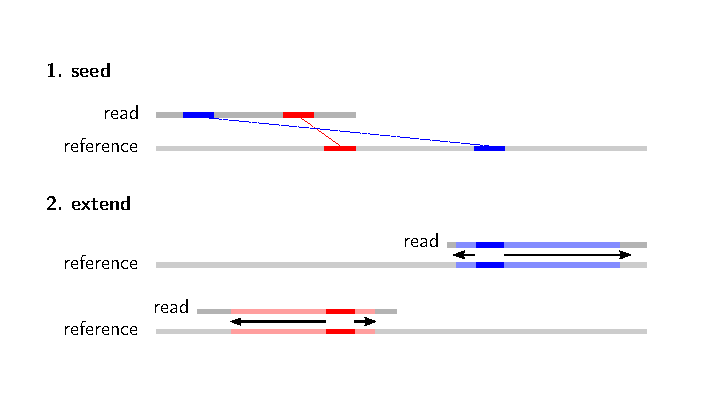
\includegraphics[width=0.8\textwidth]{figures/chap3_seedandextend}
	  \caption{}
	  \label{fig:chap3:modelneighborhood}
   \end{minipage}
\end{figure}


\subsection{Split reads and breakpoint algorithm}
Another interesting feature of our mapping algorithm is its ability to
map split reads. Split reads are sequences constituted by more
than one DNA fragment. Such reads are deliberately generated in
experiments like Hi-C \cite{}, in which the different fragments that
constitute the sequenced DNA molecule may originate from very distant
positions of the genome.

In this context, the problem generalizes to map an unknown number of
subsequences of unknown lengths. One possible way to detect the
breakpoint between two different fragments is to infer the location of
an abrupt decrease of sequence identity during alignment. In effect,
during the Needleman-Wunsch extension, one expects high identity
between the read and the reference as long as the alignment extends
over the seeded fragment. However, when the alignment reaches the
breakpoint between fragments, the rest of the extension behaves
approximately like an alignment between random sequences. We exploit
this fact and design an optimal breakpoint detection algorithm based
on the Maximum Likelihood (ML) breakpoint detection model presented in
\cite{breakpoint}. 

\begin{figure}[h]
	\begin{minipage}[b]{\linewidth}
	  \centering
	  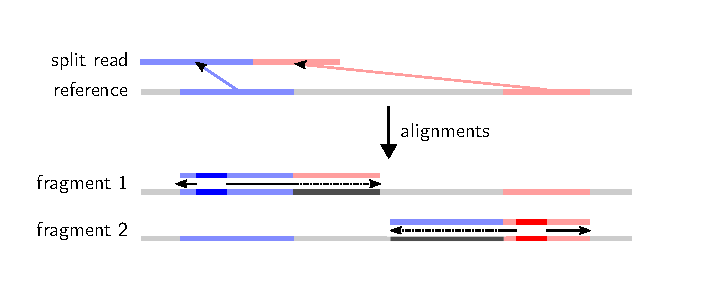
\includegraphics[width=0.8\textwidth]{figures/chap3_splitread}
	  \caption{}
	  \label{fig:chap3:modelneighborhood}
   \end{minipage}
\end{figure}

In the breakpoint detection algorithm we model our sequence as a
sequence $S = (S_1,\ldots,S_n)$, where the $S_i$ are independent
random variables following a binomial probability distribution
\begin{equation}
  \label{eq:chap3:bp-model}
  \mbox{pr}(S_i = 1) =
  \begin{cases}
    \theta_0 & (i=1,\ldots,b) \\
    \theta_1 & (i=b+1,\ldots,n)
  \end{cases}
\end{equation}
and $\mbox{pr}(R_i=0) = 1-\mbox{pr}(R_i=1)$; and $\theta_0$ and
$\theta_1$ are the known alignment mismatch probabilities but the
change-point $b$ is unknown. The random variable outputs 0 and 1
represent matches and mismatches between the read and the reference,
respectively. For our model of alignment over a split-read, we
estimate $\theta_0$ to be the expected error probability of two
truly-matching sequences, which depends on the sequencing technology
error rate, the mutation rate and the divergence of the reference text
and the real genome. We expect the value of $\theta_0$ for Illumina
reads mapped on a well annotated genome to be $\theta_0 < 0.05$. On
the other side, $\theta_1$ represents the error read past the
split-read boundary, which we approximate to a comparison of two
random sequences, being $\theta_1 > 0.35$ for an alignment with
insertions, deletions and substitutions.

Under the model \eqref{eq:chap3:bp-model}, the likelihood function of
$(S_1,\ldots,S_n)$ is
\begin{equation}
  \label{eq:chap3:bp-likelihood}
  \prod_{i=1}^b \theta_0^{S_i}(1-\theta_0)^{1-S_i} \prod_{i=b+1}^n
  \theta_1^{S_i}(1-\theta_1)^{1-S_i}
\end{equation}
so that the log likelihood conditional on $b=t$, with known $\theta_0$
and $\theta_1$, can be written as
\begin{equation}
  \label{eq:chap3:bp-loglikelihood}
  L(t) =
  \sum_{i=1}^t \left\{ S_i\log\left(\frac{\theta_0}{\theta_1}\right) +
  (1-S_i)\log\left(\frac{1-\theta_0}{1-\theta1}\right) \right\}  + 
  \sum_{i=1}^n \left\{ S_i\log{\theta_1} + (1-S_i)\log (1-\theta_1)
  \right\}
\end{equation}
Hence the maximum likelihood estimate of the breakpoint $\hat{b}$ is
the value of $t$ which maximizes the sequence
\begin{equation}
  \label{eq:chap3:max-likelihood}
  X_t =
  \sum_{i=1}^{t}\left\{S_i\log\left(\frac{\theta_0}{\theta_1}\right) +
  (1-S_i)\log\left(\frac{1-\theta_0}{1-\theta_1}\right)\right\} \qquad
(t=1,\ldots,n) 
\end{equation}

The maximization step described in \eqref{eq:chap3:max-likelihood} is
applied periodically during the alignment process to track the
position and the likelihood of a potential breakpoint. The algorithm
stops when $X_{\hat{b}}$ exceeds a defined threshold, or at the end of
the alignment otherwise. A detailed relationship between the
the breakpoint confidence and the likelihood $X_{\hat{b}}$ can be
found in \cite{breakpoint}.

\section{Mapping quality}
At this point of the algorithm we obtained many candidate mapping
positions and computed the alignment score for them. But there is
still one crucial step: to provide a mapping confidence score,
i.e. the probability that the association between the read and the
reported locus is correct. The mapping quality model is what
ultimately makes the difference between a good and an average mapper,
because the final users will process their reads and trust the
assignments based on their confidence score. Hence, the mappers should
be characterized by: (i) {\em how many of the input reads is the mapper
able to find in the reference?} (sensitivity) and (ii) {\em how many
of the high confidence mappings are actually wrong assignments?}
(false positive rate). In this section we present two simple models to
evaluate the mapping confidence, which used in combination yield
better confidence estimates compared to other widely-used mappers
\cite{bwa,bowtie}.

The mapping quality reported by our mapper is computed as:
\begin{equation}
  \label{eq:chap3:mapq}
  \mbox{MAPQ} = -10\log\left(\mbox{pr}(\mbox{wrong assignment})\right)
\end{equation}

\subsection{Alignment score model}
This widely-used mapping quality model is based on the alignment
scores of the extended seeds. The idea is simple: sort the alignment
scores of the seed extensions. The locus with highest alignment score
is considered the true mapping position of the read. In case there are
many $n_1 > 1$ best matches, each match is considered equally likely
to be the true origin of the sequence. Hence, the probability of
incorrect assignment is $\mbox{pr}(\mbox{wrong assignment}) =
1-1/n_1$. As the gap between the best and the second best alignment
scores grows, the probability that the best alignment is indeed the
correct mapping position becomes evident. In effect, this is analogous
to the neighbors model, a big gap in the alignment score indicates
that the reference sequence is somehow unique and therefore it is
unlikely that its similitude with the read is due to an artifact.

When the alignments report only one $n_1=1$ best alignment, the model
computes mapping quality relative to alignment scores $Q_A$ as an
heuristic which takes into account the difference between the best and
the second best score $\Delta_{12}$, the number of second best score
matches $n_2$ and the identity (1 minus the mismatch rate) of the best
alignment $\eta$: 
\begin{equation}
  Q_A = \mathit{f}(\eta)\cdot\left(c\Delta_{12}-10\log_{10}(n_2)\right)
\end{equation}
This model is powerful but may show substantial performance
differences depending on the sequencing technology and the reference
genome, because the parameters of the heuristic $\mathit{f}, c$ are
usually calibrated by fitting a curve on simulated data. This
model alone, however, already gives extraordinary results for
well-calibrated inputs \cite{bwa}.

\subsection{The neighbors model}
The neighbors model follows the same principle of the alignment score
model: to quantify the reliability of the read-locus assignment
through the exploration of the close neighborhood. This model,
however, is both faster and more precise thanks to the access to
exhaustive neighborhood information. That also allows a notable
reduction of necessary alignments at the extension step, since one can
assess the state of the neighborhood of a single seed extension,
whereas the same is not possible using the alignment score model, in
which at least two alignments are required.

Consider the following sequences $T_R$, $T_B$,and $T_N$, which
represent the read, the sequence in the reference that best matches
the read and its closest neighbor, respectively. $T_B$ is known and
has been obtained through a seed-and-extend process applied to
$T_R$. The closest neighbor of $T_B$ is unknown but we can infer some
information about $T_N$ using the neighborhood annotation. Since $T_B$
and $T_N$ are sequences of the reference, we will denote their
positions with $l_B$ and $l_N$. We also denote the Levenshtein
distance between two sequences $T_1$ and $T_2$ as
$\mathrm{d}(T_1,T_2)$.  

\begin{figure}[h]
	\begin{minipage}[b]{\linewidth}
	  \centering
	  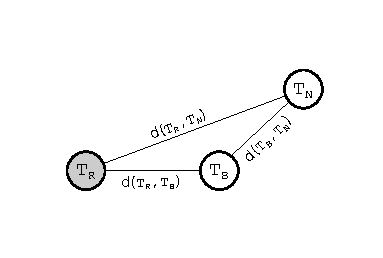
\includegraphics[width=0.5\textwidth]{figures/chap3_neighmodel_neighborhood}
	  \caption{}
	  \label{fig:chap3:modelneighborhood}
   \end{minipage}
\end{figure}

The diagram of Figure \ref{fig:chap3:modelneighborhood} illustrates the local neighborhood
composed by $T_R$, $T_B$ and $T_N$. Note, however, that this
neighborhood does not represent the annotation since, in general,
$T_R$ does not belong to the reference. The distance
$\mathrm{d}(T_R,T_B)$ is known because $T_R$ and $T_B$ had been
aligned previously during the seed-and-extend algorithm. The
distance $\mathrm{d}(T_B,T_N)$ can be obtained from the neighborhood
annotation, but the remaining distance $\mathrm{d}(T_R,T_N)$ is
generally unknown. The fact that $\mathrm{d}(T_R,T_S)$ is unknown greatly
complicates the construction of a model to evaluate the mapping
quality. The goal of the model is to estimate the probability that
$T_R$ did not originate from $T_B$, which we approximate by the
probability that $T_R$ originated from any of closest neighbors
$T_N$. To derive an estimation of such probability, we make several
reasonable assumptions on $\mathrm{d}(T_R,T_S)$: 
\begin{assumption}
  \label{chap3:assumption-seedsensitivity}
  The distance $\mathrm{d}(T_R,T_B)$ is small enough to assume
  that the whole $\mathrm{d}(T_R,T_B)$-neighborhood of $T_R$ has
  been explored during the seeding stage. In other words, we assume
  that the seeding strategy is fully sensitive up to
  $\mathrm{d}(T_R,T_B)$ mismatches.
\end{assumption}
\begin{assumption}
  \label{chap3:assumption-rndist}
  As a result of assumption \ref{chap3:assumption-seedsensitivity}, we
  conclude that $T_B$ is the closest neighbor of $T_R$ and the
  inequality $\mathrm{d}(T_B,T_N) > \mathrm{d}(T_R,T_B)$ must
  hold. Otherwise, if $\mathrm{d}(T_B,T_N) \le \mathrm{d}(T_R,T_B)$
  we would have performed a seed extension of $T_R$ on $T_B$ and
  $\mathrm{d}(T_R,T_B)$ would be known.
\end{assumption}

We start to build our model leveraging on assumptions
\ref{chap3:assumption-seedsensitivity} and
\ref{chap3:assumption-rndist}, with the hypothesis that the true
origin of $T_R$ is $l_N$ instead of $l_B$. From our definition of
mapping quality, it is reasonable to approximate the probability of
incorrect mapping by the probability that $T_R$ originated from $l_N$,
even though $T_B$ lies closer in the neighborhood space.

\begin{figure}[h]
	\begin{minipage}[b]{\linewidth}
	  \centering
	  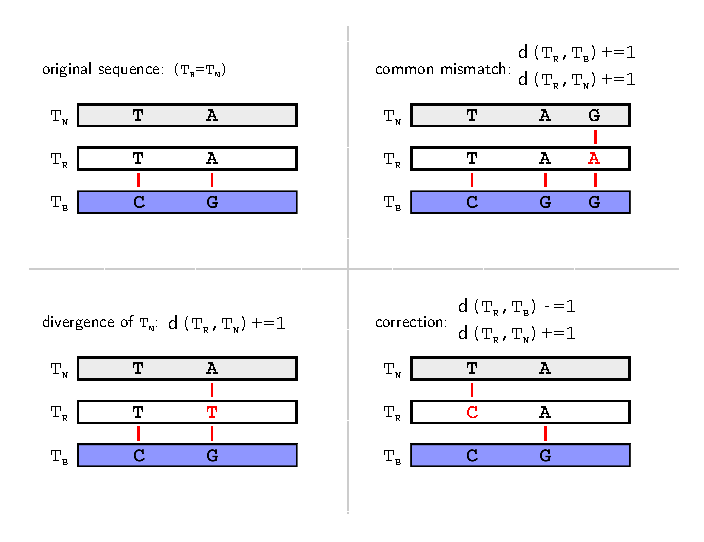
\includegraphics[width=0.7\textwidth]{figures/chap3_neigh_mutations}
	  \caption{}
	  \label{fig:chap3:mutations}
   \end{minipage}
\end{figure}

Our hypothesis concludes that the physical sequence taken from the
reference is $T_N$ but it has been exposed to modifications during the
experiments and/or the sequencing steps and the final read lies closer
to $T_B$. In Figure \ref{fig:chap3:mutations} we summarize the
possible modifications that the molecule can suffer and how do they
affect the position of the read relative to $T_N$ and $T_B$. The
top-left panel illustrates the original sequence, where $T_R$ is
copied from $T_N$, and their differences with $T_B$. The only way we
can now push $T_R$ towards $T_B$ is through nucleotide modifications,
with three possible scenarios: 
\begin{itemize}
\item The first one is the {\em common mismatch}, when the modified
  nucleotide is not a mismatch between $T_B$ and $T_N$, in this case
  the distances from both references to $T_R$ increase by one
  mismatch. 
\item The second case is when a mismatched nucleotide between $T_N$
  and $T_B$ is modified but it is not set equal to the one in
  $T_B$. So, $T_R$ {\em diverges from $T_N$} but not from $T_B$,
  because the mismatch already existed between $T_R$ and $T_B$ at that
  position.
\item The third case is the same as case 2 but the modified nucleotide
  is set to match the one in $T_B$, causing a {\em correction} with
  respect to $T_B$. In this case the distance to $T_N$ increases by
  one and $\mathrm{d}(T_R,T_B)$ is decreased by one.
\end{itemize}

Now the question is how these modification events combined to finally
situate $T_R$ closer to $T_B$. Under our hypothesis, we can express
the distances of the neighborhood in Figure
\ref{fig:chap3:modelneighborhood} as
\begin{equation}
  \begin{array}{cl}
    \label{eq:chap3:dist_mutations}
    \mathrm{d}(T_R,T_N) = & M + C + D \\
    \mathrm{d}(T_R,T_B) = & \mathrm{d}(T_B,T_N) + M - C
  \end{array}
\end{equation}
where the distances and all the other terms are non-negative: $M$ are
the common mismatches, $D$ the divergent mismatches and $C$ the
corrections. It is clear from \eqref{eq:chap3:dist_mutations} that at
least one correction or two divergences must happen to verify
$\mathrm{d}(T_R,T_B) < \mathrm{d}(T_R,T_N)$, which represents
Assumption \ref{chap3:assumption-rndist}, and can be rewritten as
follows:
\begin{equation}
  \label{eq:chap3:rndist_mutations}
  \mathrm{d}(T_B,T_N) + M - C < M + C + D
\end{equation}
which, simplified yields
\begin{equation}
  \label{eq:chap3:rndist_mutations_simp}
  \mathrm{d}(T_B,T_N) < 2C + D
\end{equation}
where, in effect, for the smallest distance $\mathrm{d}(T_B,T_N)=1$ we
need $C\ge1$ or $D\ge2$.

%Si d(B,N) no es conegut, s'assumeix que la distancia que recorre T_R
%es la minima, es a dir, ceil(d(B,N)/2). De la combinatoria de les
%possibles mutacions es treu la probabilitat d'error.

%Explicar al final de tot que les anotacions es fan per $k$ concretes,
%i que per avaluar aixo, si la longitud de la sequencia no coincideix
%amb cap $k$, s'agafa el tros de sequencia mes gran possible amb un
%dels valors de $k$ disponibles.




\chapter{Results}

The mapping performance of our algorithm is tested and discussed in
this chapter. The results of our mapper are consistently compared with
two of the most widely used mappers: \texttt{bwa-mem} \cite{bwa} and
\texttt{bowtie2} \cite{bowtie}. The performance of the three mappers
has been tested on simulated Human and Drosophila Illumina data
generated with wgsim (http://github.com/lh3/wgsim). 

Datasets of 1 illion of single-end 50bp reads were generated for
different sequencing error rates. Namely, we considered three
usual sequencing scenarios: good (1\% error rate), standard (2\%) and
average (5\%). Wgsim was run in command line with parameters
\texttt{-e R -N 1000000 -1 50 -2 0}, where \texttt{R} was set to
$0.01$, $0.02$ or $0.05$ depending on the scenario. The simulated
reads are presented in fastq format without meaningful quality
information (all bases are assigned the same quality score). The
sequence headers contain the real locus and the strand of the
read. After running the three mapping algorithms on the datasets the
read headers are parsed and compared to the mapped locus and
strand. Reads are considered well mapped if the estimate in the same
strand and within 100 basepairs of the actual locus.

The algorithms were benchmarked on a dual-processor Intel Xeon
E5-2687W v2 system with 256GB of DDR3-RAM at 1866~Mhz. All softwares
were set to run single-core. Our mapper and \texttt{bwa-mem} were ran
using default parameters, \texttt{bowtie2} was setup to use the
\texttt{very-sensitive} configuration. 

Our benchmark includes three measurements:
\begin{itemize}
  \item {\bf Sensitivity} expressed as the fraction of correctly mapped
    reads with respect to the total input read count.
  \item {\bf Positive error rate} is the rate of false positives per true
    positive.
  \item {\bf Throughput} expressed as the rate of true positives per second.
\end{itemize}

We believe that these three magnitudes provide a good characterization
of the performance of a mapper. Almost all benchmarks evaluate the
sensitivity, but it is equally important to provide an accurate
estimate of the expected number of incorrect mappings for each quality
score. This will ultimately help the users decide which quality score
threshold is better suited for their needs. We combine these
magnitudes in two-dimensional plots to show the comparison of
sensitivity versus positive error rate, and throughput versus positive
error rate. The first provides valuable information to tune the
acceptable quality threshold, clearly showing how many correct
mappings one must disregard in order to reduce the false positive
rate. The latter is a representation of how efficiently the
computational power is spent.

\subsubsection{Classification performance}

The classification and mapping performence achieved by the different
algorithms is represented in Figure \ref{fig:chap4:hg}.1. This result
compares the sensitity versus the false positive rate achieved in the
Human datasets with $1\%$ (left), $2\%$ and $5\%$ error rate. Each
point represents the values for a different mapping quality threshold,
i.e. a threshold on mapping quality is applied on the mapping output
and all the reads below the threshold are discarded. The sensitivity
and false positive rates are therefore measured  with the reads whose
quality is above the threshold. This process is repeated for all the
possible quality values, starting from 0 (the rightmost points). The
general trend of the mappers is the one expected: the false positive
rate decreases as the quality increases, but so does the sensitivity.

Our algorithm outperforms the \texttt{bwa-mem} and \texttt{bowtie2} in
the three configurations, achieving a good response even in the worst
configuration. Remarkably, our algorithm consistently reports 100.000
more well-mapped sequences with false positive rates below $10^{-4}$
at the standard Illumina setting (2\%). Moreover, our mapper shows a
smooth response on average sequencing (5\% error), recovering $>65\%$
of the reads in all the possible configurations, whereas the other
mappers drop well below $50\%$ as soon as they reach a false positive
rate of $10^{-4}$.

\begin{figure}[h]
	\begin{minipage}[b]{0.5\linewidth}
	  \centering
	  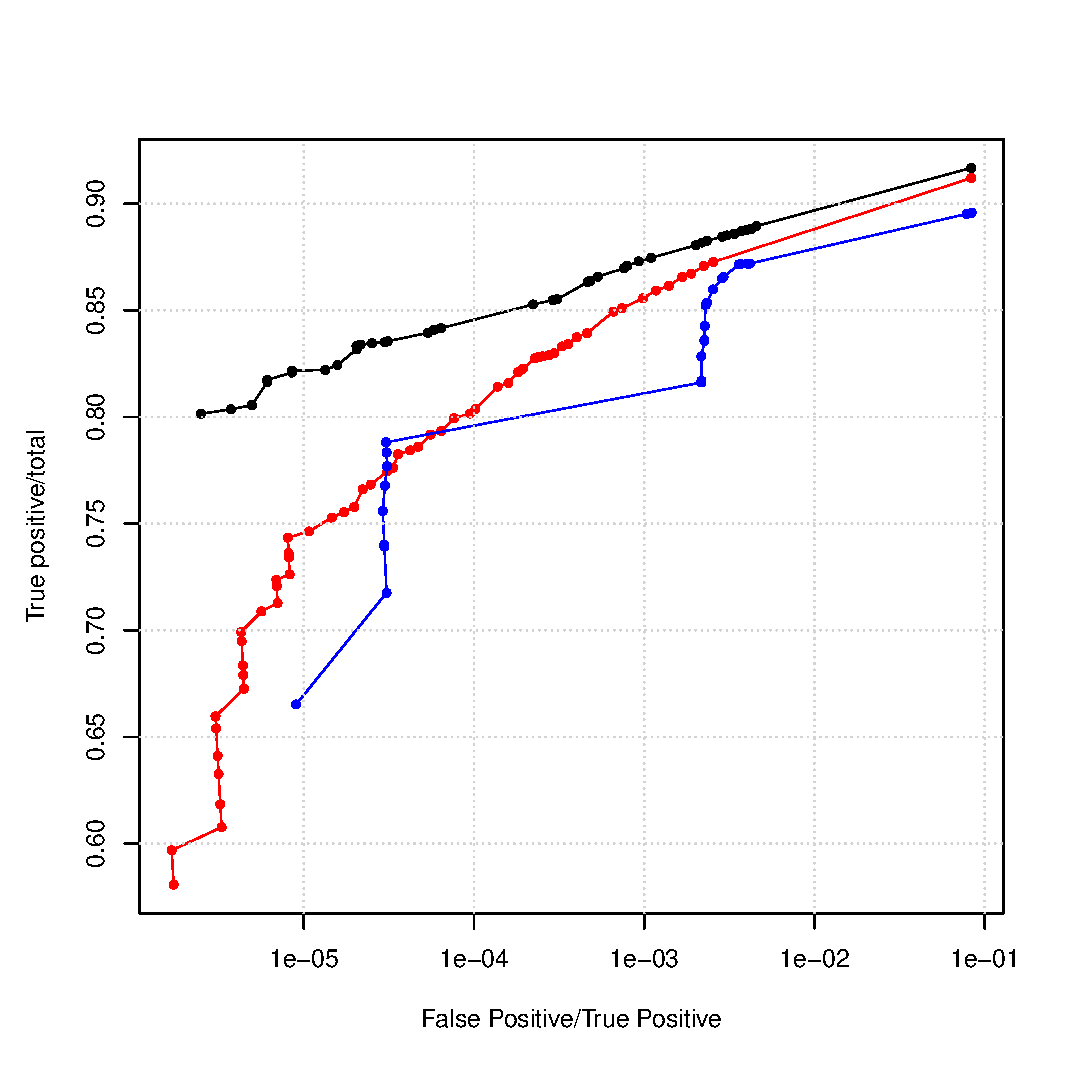
\includegraphics[width=\textwidth]{figures/chap4_hg_1_15}
   \end{minipage}
	\begin{minipage}[b]{0.5\linewidth}
	  \centering
	  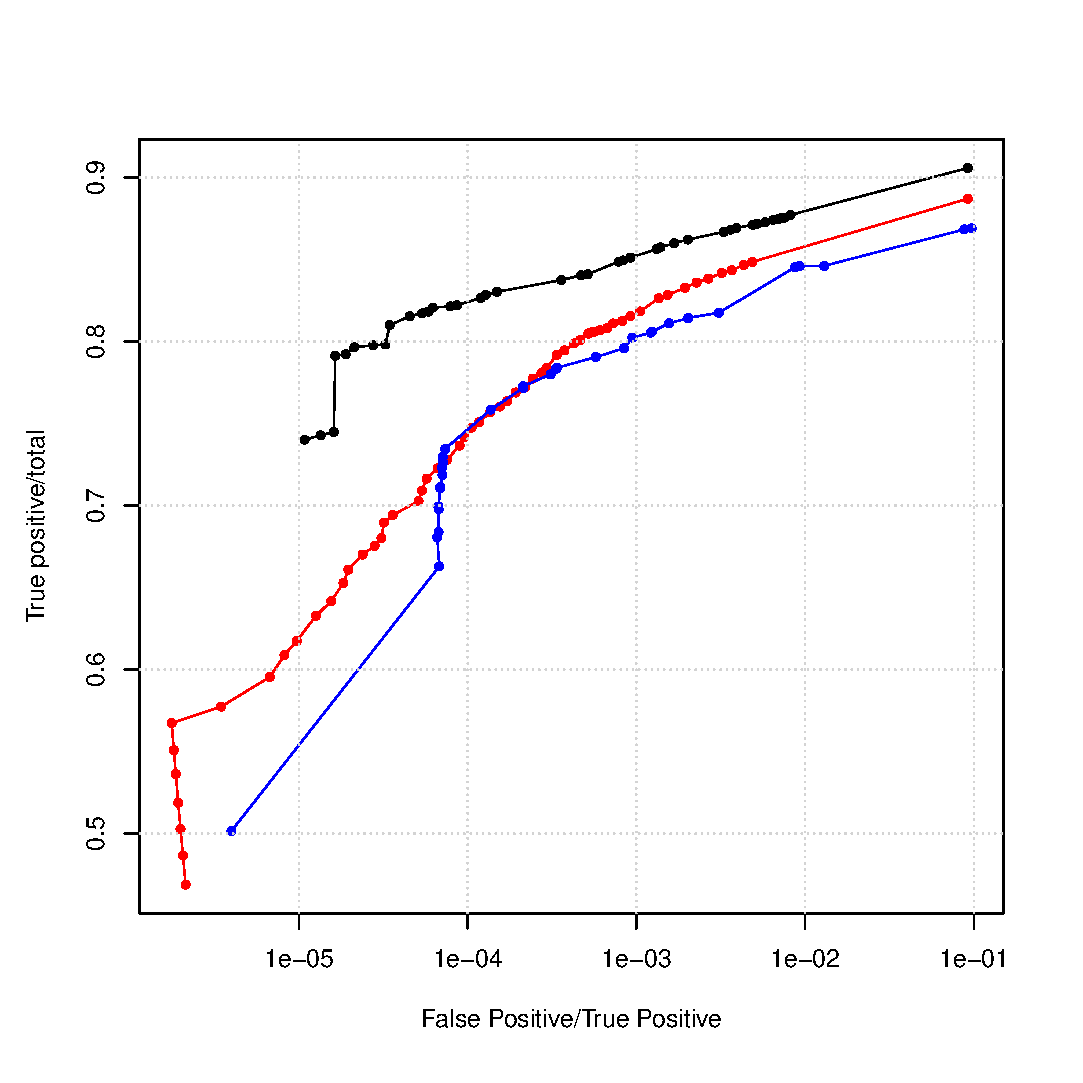
\includegraphics[width=\textwidth]{figures/chap4_hg_2_15}
   \end{minipage}
	\begin{minipage}[b]{\linewidth}
	  \centering
	  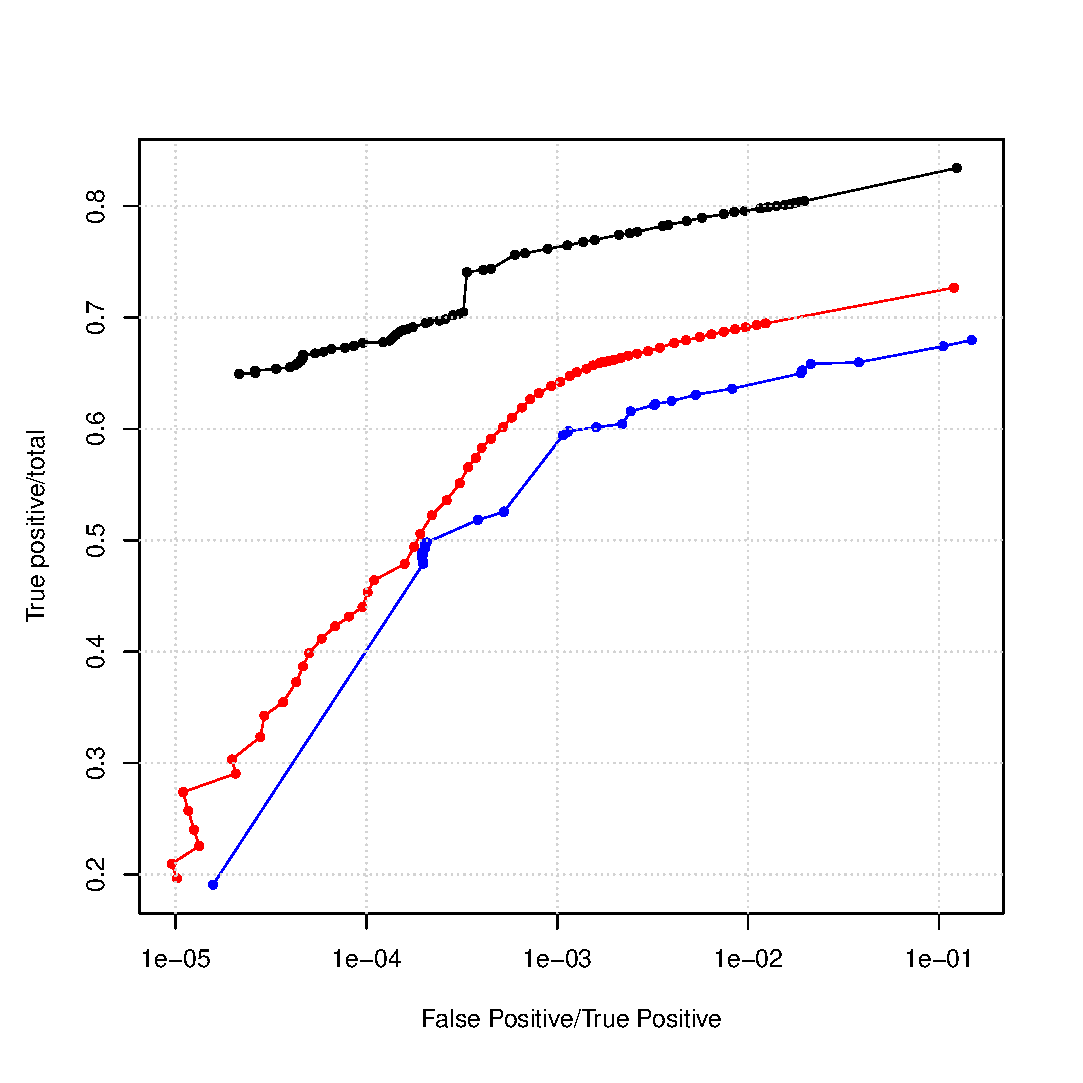
\includegraphics[width=0.5\textwidth]{figures/chap4_hg_5_15}
   \end{minipage}
   \label{fig:chap4:hg}
  \caption{Sensitivity vs error rate for all the possible mapping
       quality thresholds. Illumina simulated reads on Human Genome
       v19, with 1\% (left), 2\% (right) and 5\% (bottom) error
       rate. Comparison between bowtie2 (blue), bwa-mem (red) and our
       mapper (black).} 
\end{figure}

\subsubsection{Computational efficiency}

In this section we assess the computational efficiency of the
algorithms. To do so, we measure the rate of true positives produced
at the output for a target error read. We prefer a direct measurement
of how well the computational resources are spent rather than the
absolute running time, since an algorithm may run very fast but
produce poor results. The measurements of computational efficiency are
shown in Figure \ref{fig:chap4:hg}.1 for Human Genome reads in
the two extreme cases of 1\% error rate (left) and 5\% error rate
(right). We expect the algorithms to perform faster when the data
contains few errors, because the seeding is more effective and it is
more likely that a few alignments will suffice to produce an
estimate. This is what we observe if we compare the average true
positive rates. All the algorithms perform faster when the error rate
is small. On the other side, our algorithm takes advantage of the seed
significance filter to speed up the mapping process when the seed is
considered highly significant, which happens more often if the read
quality is good. On the other side, for 5\% error, both bwa-mem and
bowtie2 outperform our mapper for false positive rates above
$10^{-4}$. Hence, the good performance of our mapper observed in
Figure \ref{fig:chap4:hg-rate}.2 is at the expense of a decreased
computational efficiency. This lower computational efficiency at high
error rate is attributed to the time spent processing difficult
reads. The difficult reads, which contain many errors, take orders of
magnitude longer to map because they can only be mapped using
high-sensitivity seeding strategies.

\begin{figure}[h]
   \label{fig:chap4:hg-rate}
	\begin{minipage}[b]{0.5\linewidth}
	  \centering
	  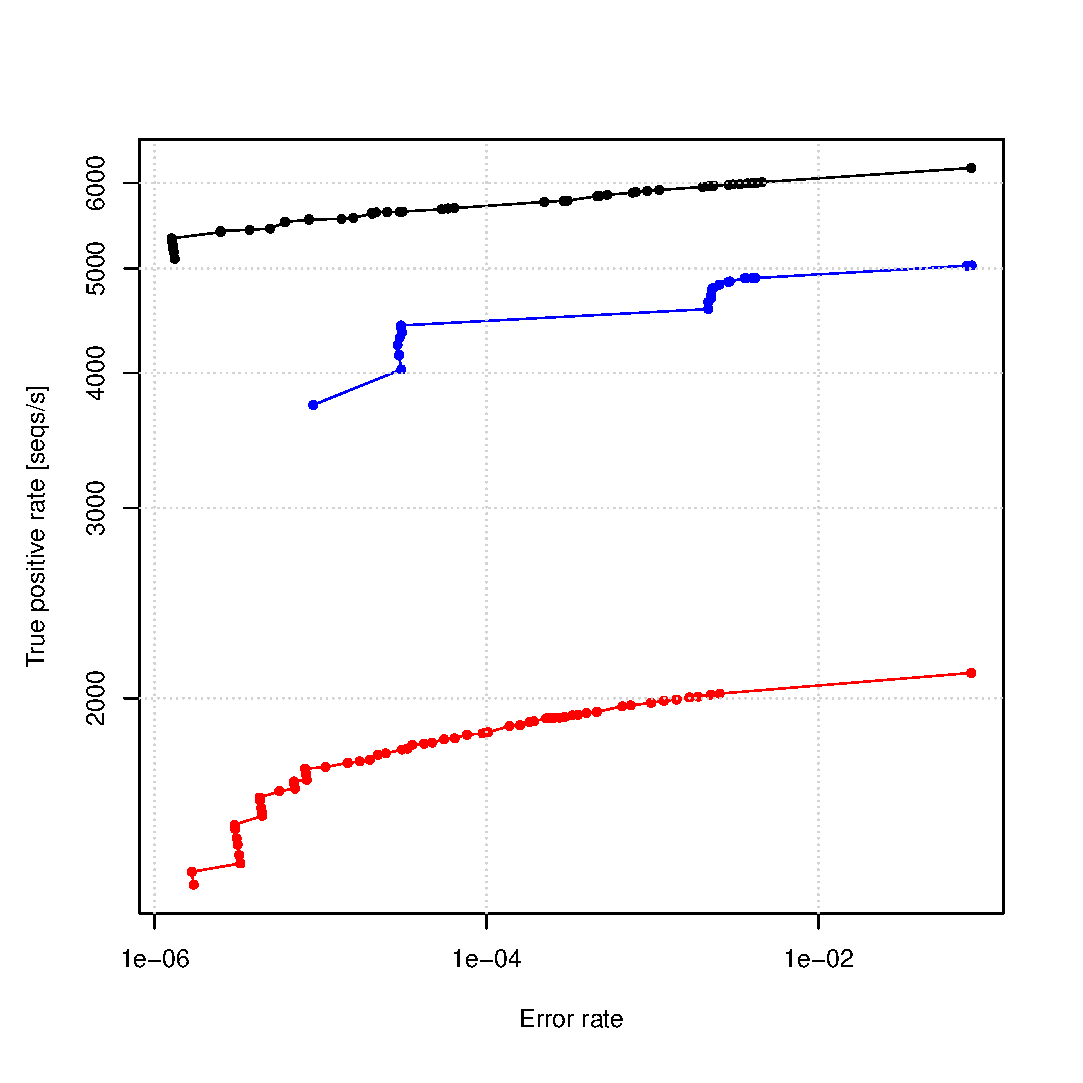
\includegraphics[width=\textwidth]{figures/chap4_hg_1_15_throughput}
   \end{minipage}
	\begin{minipage}[b]{0.5\linewidth}
	  \centering
	  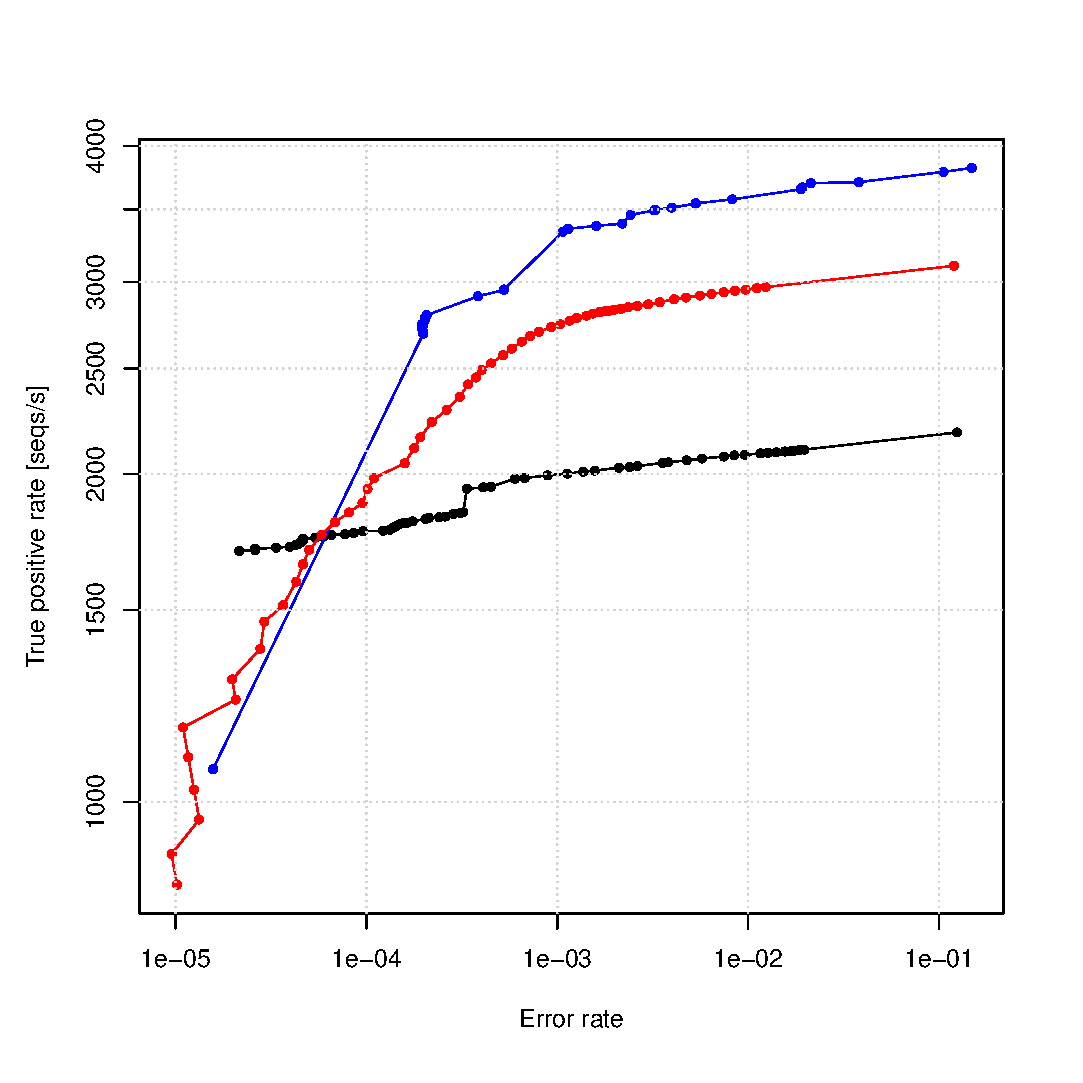
\includegraphics[width=\textwidth]{figures/chap4_hg_5_15_throughput}
   \end{minipage}
   \caption{Throughput (correctly mapped sequences per core per
       second) vs error rate for all the possible mapping quality
       thresholds. Illumina simulated reads on Human Genome v19, 1\%
       (left) and 5\% (right) error rate. Comparison between bowtie2
       (blue), bwa-mem (red) and our mapper (black). }
\end{figure}

\subsubsection{Other genomes}

We have also benchmarked the mappers on a different reference:
Drosophila Melanogaster. Figure \ref{fig:chap4:dmel}.3 summarizes the
same results shown in Figure \ref{fig:chap4:hg115} for error rates of
2\% and 5\%. The results show the same trend as in the Human genome,
but all the algorithms show diminished sensitivity at the highest
mapping qualities. This is due to the nature of the genome and
generally indicates that the repeats have more copies compared to the
average number in the Human genome. 

\begin{figure}[h]
   \label{fig:chap4:dmel}
	\begin{minipage}[b]{0.5\linewidth}
	  \centering
	  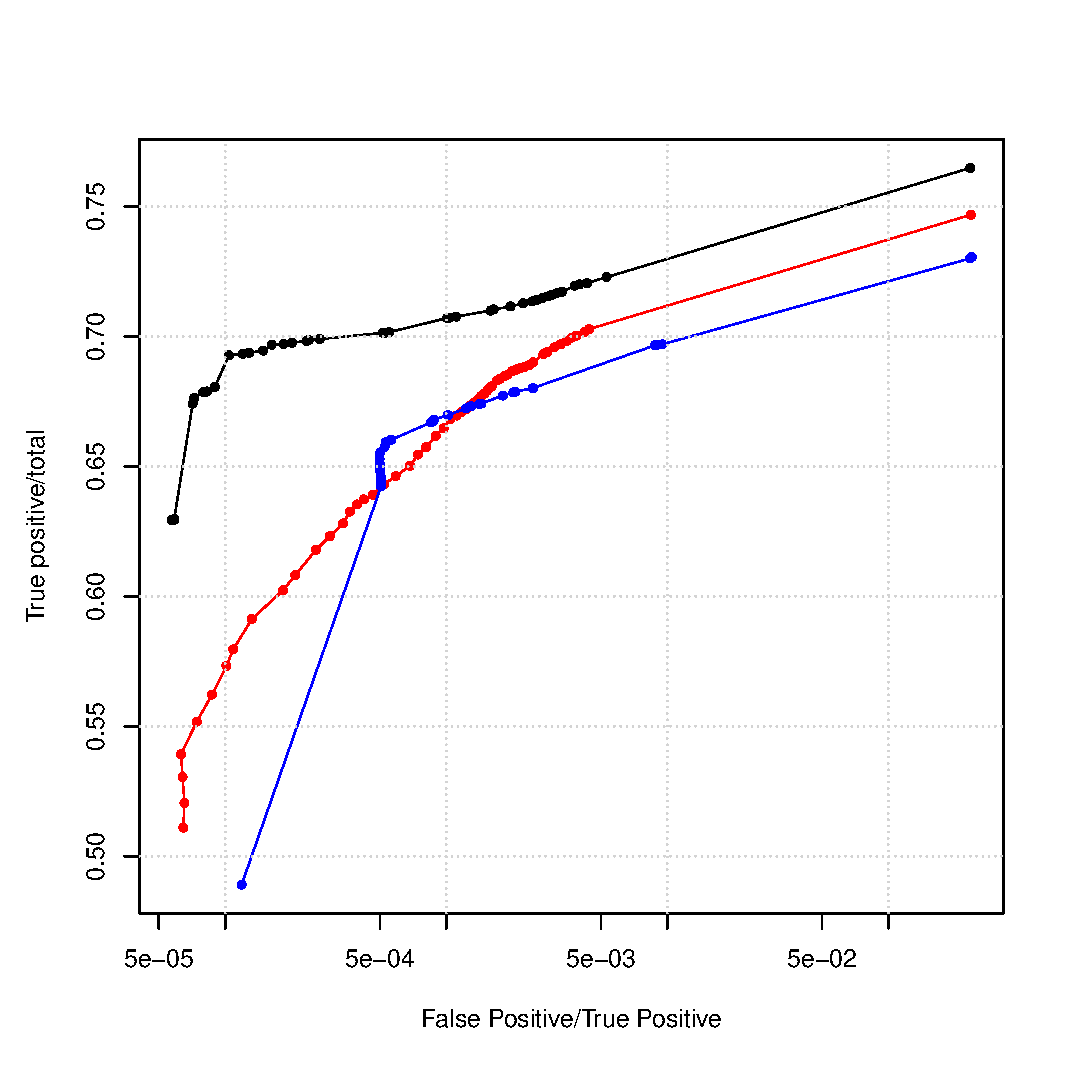
\includegraphics[width=\textwidth]{figures/chap4_dmel_2_15}
   \end{minipage}
	\begin{minipage}[b]{0.5\linewidth}
	  \centering
	  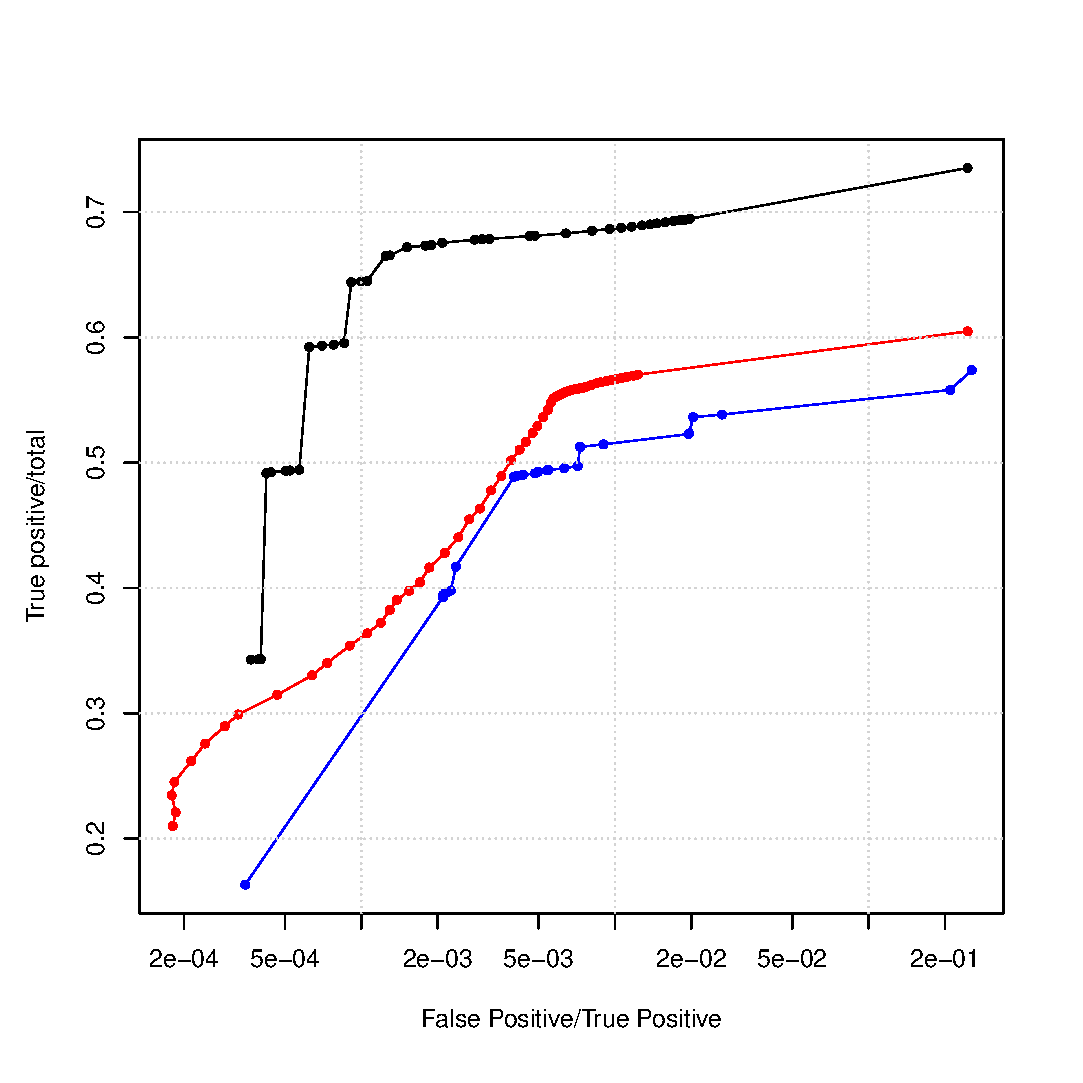
\includegraphics[width=\textwidth]{figures/chap4_dmel_5_15}
   \end{minipage}
   \caption{Sensitivity vs error rate for all the possible mapping
       quality thresholds. Illumina simulated reads on Drosophila
       Melanogaster genome v3, 2\% (left) and 15\% (right) error
       rate. Comparison between bowtie2 (blue), bwa-mem (red) and our
       mapper (black). } 

\end{figure}

\chapter{Conclusions and future work}

Overall, we have shown that even though the current mapping algorithms
have good performance, there is still room for
innovation. Complementing the search indices with annotations of 
genomic features, such as the $k$-mer neighborhood can enhance the
overall performance and efficiency of the algorithm. It also provides
greater control on the output because the use of statistical models,
like the one presented, can be exploited to recursively evaluate the
computational cost of the on-going computation. In this work, we have
only shown a very simple and straightforward use of the neighborhood
model. To better characterize the advantages of this annotation, we
would have to evaluate its performance in a more extensive benchmark,
with varying sequence lengths, error rates and other sequencing
technologies. For our purpose, this mapper was ideated as a previous
step to build a split-read mapper for Hi-C reads. Therefore, our goal
was to achieve high sensitivity and improved quality score assignment on
short reads, with running times comparable to the state-of-the-art
mappers. In this sense, we have clearly succeeded.

The next steps would be to improve the mapper to work reliably with
the latest sequencing technologies (PacBio and ), which produce reads
on the order of kilobasepairs long, but at the expense of a much
higher error rate (around 15\%). To do so, we would need to generalize
the Neighbor model to greater neighborhood spaces, in which Assumptions
\ref{} and \ref{} of Section \ref{} may not hold. Other future tasks
include the design of optimized decisions based on the seed
significance to increase even more the computational efficiency.
